\documentclass{article}


\usepackage{hyperref}
\hypersetup{
    colorlinks,
    citecolor=black,
    filecolor=black,
    linkcolor=black,
    urlcolor=black
}

\usepackage{graphicx}
\usepackage{tikz}
\usepackage[framemethod=TikZ]{mdframed}
\usepackage{geometry}
\usepackage{amsmath}
\usepackage{amssymb}
\usepackage{amsfonts}
\usepackage{scrextend}
\usepackage{enumitem, multicol}
\usepackage{caption}
\usepackage{ifthen}
\usepackage{changepage}
\usepackage{listings}
\usepackage{tikz-cd}
\usetikzlibrary{arrows.meta, automata, 
                positioning, 
                quotes}
\usepackage{amsmath}
\usepackage[low-sup]{subdepth}
\usepackage{ebproof}
\usepackage{mdframed}
\usepackage{calc}
\usepackage{mathtools}
\usepackage{forest}
\usepackage[dvipsnames]{xcolor}


\newlength\twound
\settowidth{\twound}{\_}
\newcommand{\dunder}{\rule{2\twound}{0.4pt}}

\newcommand*{\fullref}[1]{\hyperref[{#1}]{\ref*{#1} \nameref*{#1}}}

\DeclarePairedDelimiter{\ceil}{\lceil}{\rceil}

\DeclarePairedDelimiter{\encode}{\ulcorner}{\urcorner}


\makeatletter
\newsavebox{\@brx}
\newcommand{\llangle}[1][]{\savebox{\@brx}{\(\m@th{#1\langle}\)}%
  \mathopen{\copy\@brx\kern-0.5\wd\@brx\usebox{\@brx}}}
\newcommand{\rrangle}[1][]{\savebox{\@brx}{\(\m@th{#1\rangle}\)}%
  \mathclose{\copy\@brx\kern-0.5\wd\@brx\usebox{\@brx}}}
\makeatother

\lstset{
    basicstyle=\ttfamily,
    mathescape=true,          % Enable math mode inside listings
    columns=fullflexible      % Ensure spacing is preserved
}

\newmdenv[
  topline=false,
  bottomline=false,
  rightline=false,
  skipabove=\topsep,
  skipbelow=\topsep
]{siderules}

\def\axiom{\infer0}

\usetikzlibrary{calc}
% `pathmorphing` is necessary to draw squiggly arrows.
\usetikzlibrary{decorations.pathmorphing,shapes.misc}


% A TikZ style for curved arrows of a fixed height, due to AndréC.
\tikzset{curve/.style={settings={#1},to path={(\tikztostart)
    .. controls ($(\tikztostart)!\pv{pos}!(\tikztotarget)!\pv{height}!270:(\tikztotarget)$)
    and ($(\tikztostart)!1-\pv{pos}!(\tikztotarget)!\pv{height}!270:(\tikztotarget)$)
    .. (\tikztotarget)\tikztonodes}},
    settings/.code={\tikzset{quiver/.cd,#1}
        \def\pv##1{\pgfkeysvalueof{/tikz/quiver/##1}}},
    quiver/.cd,pos/.initial=0.35,height/.initial=0}

% TikZ arrowhead/tail styles.
\tikzset{tail reversed/.code={\pgfsetarrowsstart{tikzcd to}}}
\tikzset{2tail/.code={\pgfsetarrowsstart{Implies[reversed]}}}
\tikzset{2tail reversed/.code={\pgfsetarrowsstart{Implies}}}
% TikZ arrow styles.
\tikzset{no body/.style={/tikz/dash pattern=on 0 off 1mm}}

\definecolor{dkgreen}{rgb}{0,0.6,0}
\definecolor{darkred}{rgb}{0.55,0,0}
\definecolor{gray}{rgb}{0.5,0.5,0.5}
\definecolor{mauve}{rgb}{0.58,0,0.82}

%\usetikzlibrary{decorations.markings}

\geometry{
 a4paper,
 total={170mm,257mm},
 left=30mm,
 top=25mm,
}

\newcommand{\indrule}[3]{\ifstrempty{#1}{\mathrel{\raisebox{6pt}{\(\dfrac{#2}{#3}\)}}}{\mathrel{\raisebox{6pt}{(\text{#1})\ \ \(\dfrac{#2}{#3}\)}}}}
\newcommand{\eqdef}{\overset{\text{def}}{=}}

\definecolor{darkblue}{rgb}{0,0,0.55}

\newcounter{quest}\setcounter{quest}{0}
\renewcommand{\thequest}{\arabic{quest}}
\newenvironment{quest}[1][]{%
\ifstrempty{#1}%
{%
\refstepcounter{quest}%
\mdfsetup{%
frametitle={%
\tikz[baseline=(current bounding box.east),outer sep=0pt]
\node[anchor=east,rectangle,fill=darkblue!20]
{\strut Question~\thequest.};}}
%
}%
{
\ifthenelse{\equal{#1}{a} \OR \equal{#1}{i} \OR \equal{#1}{1}}{\refstepcounter{quest}}{}
\mdfsetup{%
frametitle={%
\tikz[baseline=(current bounding box.east),outer sep=0pt]
\node[anchor=east,rectangle,fill=darkblue!20]
{\strut Question~\thequest.#1)};}}%
}%
\mdfsetup{innertopmargin=10pt,linecolor=darkblue!20,%
linewidth=2pt,topline=true,%
frametitleaboveskip=\dimexpr-\ht\strutbox\relax
}
\begin{mdframed}[]\relax%
}{\end{mdframed}}



\setlength{\parindent}{0px}

\usetikzlibrary{decorations.markings}


\geometry{
 a4paper,
 total={170mm,257mm},
 left=30mm,
 top=25mm,
}


\newcommand{\R}{\mathbb{R}}
\newcommand{\pdv}[2]{\frac{\partial #1}{\partial #2}}
\newcommand{\lbold}[1]{\textbf{\large{ #1}}}
\newcommand{\minus}{\scalebox{1.0}[1.0]{\(-\)}}
\newcommand{\boldminus}{\(\boldsymbol{-}\)}
\newcommand{\addtopstrut}{\rule[5pt]{0pt}{.7\baselineskip}}%
\newcommand{\addbottomstrut}{\rule[-5pt]{0pt}{0pt}}%

\newcounter{theo}[section]\setcounter{theo}{0}
\renewcommand{\thetheo}{\arabic{section}.\arabic{theo}}
\newenvironment{theo}[2][]{%
\refstepcounter{theo}%
\ifstrempty{#1}%
{\mdfsetup{%
frametitle={%
\tikz[baseline=(current bounding box.east),outer sep=0pt]
\node[anchor=east,rectangle,fill=red!20]
{\strut Theorem~\thetheo};}}
}%
{\mdfsetup{%
frametitle={%
\tikz[baseline=(current bounding box.east),outer sep=0pt]
\node[anchor=east,rectangle,fill=red!20]
{\strut Theorem~\thetheo:~#1};}}%
}%
\mdfsetup{innertopmargin=10pt,linecolor=red!20,%
linewidth=2pt,topline=true,%
frametitleaboveskip=\dimexpr-\ht\strutbox\relax
}
\begin{mdframed}[]\relax%
\label{#2}}{\end{mdframed}}

\definecolor{pastelgreen}{RGB}{193, 225, 193}

\newcounter{lem}[section]\setcounter{lem}{0}
\renewcommand{\thelem}{\arabic{section}.\arabic{lem}}
\newenvironment{lem}[2][]{%
\refstepcounter{lem}%
\ifstrempty{#1}%
{\mdfsetup{%
frametitle={%
\tikz[baseline=(current bounding box.east),outer sep=0pt]
\node[anchor=east,rectangle,fill=pastelgreen]
{\strut Lemma~\thelem};}}
}%
{\mdfsetup{%
frametitle={%
\tikz[baseline=(current bounding box.east),outer sep=0pt]
\node[anchor=east,rectangle,fill=pastelgreen]
{\strut Lemma~\thelem:~#1};}}%
}%
\mdfsetup{innertopmargin=10pt,linecolor=pastelgreen,%
linewidth=2pt,topline=true,%
frametitleaboveskip=\dimexpr-\ht\strutbox\relax
}
\begin{mdframed}[]\relax%
\label{#2}}{\end{mdframed}}

\definecolor{darkblue}{rgb}{0,0,0.55}

\newcounter{defin}[section]\setcounter{defin}{0}
\renewcommand{\thedefin}{\arabic{section}.\arabic{defin}}
\newenvironment{defin}[2][]{%
\refstepcounter{defin}%
\ifstrempty{#1}%
{\mdfsetup{%
frametitle={%
\tikz[baseline=(current bounding box.east),outer sep=0pt]
\node[anchor=east,rectangle,fill=darkblue!20]
{\strut Definition~\thedefin};}}
}%
{\mdfsetup{%
frametitle={%
\tikz[baseline=(current bounding box.east),outer sep=0pt]
\node[anchor=east,rectangle,fill=darkblue!20]
{\strut Definition~\thedefin:~#1};}}%
}%
\mdfsetup{innertopmargin=10pt,linecolor=darkblue!20,%
linewidth=2pt,topline=true,%
frametitleaboveskip=\dimexpr-\ht\strutbox\relax
}
\begin{mdframed}[]\relax%
\label{#2}}{\end{mdframed}}

\newcounter{prf}[section]\setcounter{prf}{0}
\renewcommand{\theprf}{\arabic{section}.\arabic{prf}}
\newenvironment{prf}[2][]{%
\refstepcounter{prf}%
\ifstrempty{#1}%
{\mdfsetup{%
frametitle={%
\tikz[baseline=(current bounding box.east),outer sep=0pt]
\node[anchor=east,rectangle,fill=red!20]
{\strut Proof~\theprf};}}
}%
{\mdfsetup{%
frametitle={%
\tikz[baseline=(current bounding box.east),outer sep=0pt]
\node[anchor=east,rectangle,fill=red!20]
{\strut Proof~\thetheo:~#1};}}%
}%
\mdfsetup{innertopmargin=10pt,linecolor=red!20,%
linewidth=2pt,topline=true,%
frametitleaboveskip=\dimexpr-\ht\strutbox\relax
}
\begin{mdframed}[]\relax%
\label{#2}}{\end{mdframed}}



\setlength{\parindent}{0px}

\tikzset{
  ctrlpoint/.style={%
    draw=gray,
    circle,
    inner sep=0,
    minimum width=1ex,
  }
}

% cSpell:disable

\newcommand\Bezier[4]{% \bezier (lowercase 'b') was already defined elsewhere
  \node (p1) [ctrlpoint,label=90:\(P_1\)] at (#1) {};
  \node (p2) [ctrlpoint,label=90:\(P_2\)] at (#2) {};
  \node (p3) [ctrlpoint,label=90:\(P_3\)] at (#3) {};
  \node (p4) [ctrlpoint,label=90:\(P_4\)] at (#4) {};
  \draw [gray] (p1) -- (p2) -- (p3) -- (p4);
  \draw [blue] (#1) .. controls (#2) and (#3) .. (#4);
}

% cSpell:enable



\title{Further Graphics}
\author{Simon}
\begin{document}
\maketitle

\tableofcontents
\newpage

\section{Geometry Representations}

\subsection{Considerations}

When deciding on which representation to use there are a few considerations that are prevalent.

\begin{itemize}[itemsep=-4px, label={--}]
    \item \textbf{Storage}
    \item Ease of \textbf{Acquisition}
    \item Ease of \textbf{Creation} in software
    \item Ease of \textbf{Editing} features
    \item Ease of \textbf{Rendering}
\end{itemize}

\subsection{Parametric Curves \& Surfaces}

\begin{defin}[Parametric Curves \& Surfaces]{thm:parametric-curves-surfaces}
    A parametric object is one which has the general equation below for \(m,n \in \mathbb{N}\)
    \[
        f: X \rightarrow Y
    \]
    \[
        X \subseteq \R^m, \ Y \subseteq \R^n
    \]
\end{defin}

\subsubsection{Parametric Curves}

\begin{defin}[Parametric Curves]{thm:parametric-curves}
    \textbf{Parametric Curves} are when \(m=1\) and \(n \in \mathbb{N} \ \cap \ n > 1\).

    \begin{gather*}
        f: X \rightarrow Y \\
        X \subseteq \mathbb{R}, \ Y \subseteq \R^n
    \end{gather*}

    \textbf{Planar Curves} have \(n\) as 2, and similarly curves in 3D have \(n\) as 3.
\end{defin}


Planar Curves have have two functions one for each basis (or axis) \(x(t)\) and \(y(t)\) for a parameter \(t\)
\[
    f: X \rightarrow Y, \quad X \subseteq \mathbb{R},\ Y \subseteq \mathbb{R}^2
\]
\[
    \mathbf{p}(x(t),\ y(t))
\]

For example a circle can be described with \(x(t) = r \cos t\) and \(y(t) = r \sin t\) where \(t\) is the parameter,
{\(t \in [0,\, 2\pi)\)} and \(r\) is the radius of the circle.
\begin{center}
    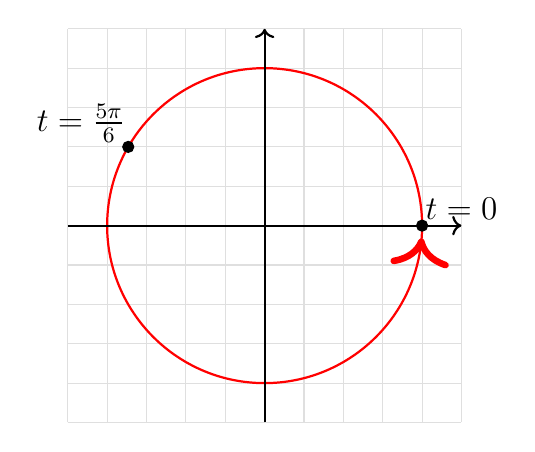
\begin{tikzpicture}[scale=0.5]
        \coordinate (A) at (4,0);
        \coordinate (B) at (4*cos{150}, 4*sin{150});
        \draw[lightgray!50] (-5, -5) grid (5, 5);
        \draw[thick, red, decoration={markings, mark=at position 0.987 with {\pgftransformscale{3}\arrow{>}}},
        postaction={decorate}] (0,0) circle[radius = 4];
        \draw[->, thick] (0, -5) -- (0, 5);
        \draw[->, thick] (-5, 0) -- (5, 0);
        \draw (A) circle[radius=4pt];
        \fill (A) circle[radius=4pt];
        \draw (B) circle[radius=4pt];
        \fill (B) circle[radius=4pt];
        \node[xshift=0.5cm, yshift=0.22cm] at (A) {\large \(t=0\)};
        \node[xshift=-0.6cm, yshift=0.3cm] at (B) {\large \(t= \frac{5\pi}{6}\)};
    \end{tikzpicture}
\end{center}

To define a curve in 3D we need \(3\) functions, one for each axis.
\[
    f: X \rightarrow Y,\quad X \subseteq \mathbb{R},\ Y \subseteq \mathbb{R}^3
\]
\[
    \mathbf{p}(t) = (x(t),\ y(t),\ z(t))
\]

\newpage
\subsubsection{Parametric Surfaces}

\begin{defin}[Parametric Surfaces]{thm:parametric-surface}
    A \textbf{Parametric Surface} is a surface in \(\R^{3}\) which is defined by a parametric equation with 
    two parameters typically \(u\) and \(v\), and from the general form \(m = 2, n = 3\).

    \[
        f: X \rightarrow Y, \quad X \subseteq \mathbb{R}^2,\ Y \subseteq \mathbb{R}^3
    \]

    \[
        \mathbf{p}(u,v) = (x(u,v), \ y(u,v), \ z(u,v))
    \]

\end{defin}

By setting \(m=2\) there are now \(2\) degrees of freedom, which allows us to define a surface.
Denoting the parameter space with \(u\) and \(v\) (known as \(uv\)-space), each point on the
surface is given by the functions \(x\), \(y\), \(z\).

\[\mathbf{p}(u,v) = (x(u,v), y(u,v), z(u,v))\]

\begin{figure}[!ht]
    \centering
    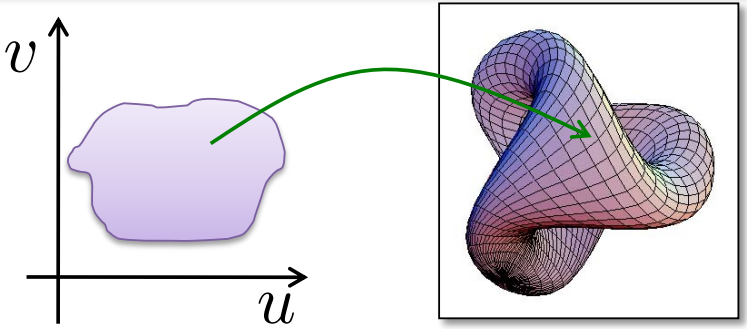
\includegraphics[width=0.5\linewidth]{images/3d_surface.png}
\end{figure}

Locally a surface is a plane which means there are only \(2\) orthogonal directions you can go to 
still stay on the surface and the other orthogonal direction will take
you either inside or outside the surface, so basically moving in the \(v\)-direction will move
you in one tangent direction and moving in the \(u\)-direction will move you in the other.

\vspace{30px}

The tangent plane for a point contains the vectors computed by taking the derivatives
w.r.t \(u\) and \(v\) as previously stated that moving in one either \(u\) or \(v\) is a tangent direction
so the partial derivative of both will be in the tangent plane.

\vspace{5px}

The surface normal \(\mathbf{n}\) is then the vector orthogonal to the tangent plane.
\vspace{30px}
\begin{center}
    \begin{minipage}{0.4\textwidth}\raggedleft
        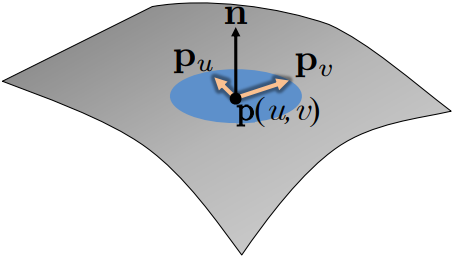
\includegraphics[width=1\linewidth]{images/surface_normal.png}
    \end{minipage}
    \begin{minipage}{0.5\textwidth}
        \[\mathbf{p}_u = \pdv{\mathbf{p}(u,v)}{u},\;
        \mathbf{p}_v = \pdv{\mathbf{p}(u,v)}{v}\]
        \hspace{20px} Regular parametrization:
        \[\mathbf{p}_u \times \mathbf{p}_v \neq \underline{0}\]
        \[\mathbf{\hat{n}}(u,v) = \frac{\mathbf{p}_u \times \mathbf{p}_v}{||\mathbf{p}_u \times \mathbf{p}_v||}\]
    \end{minipage}
\end{center}

\newpage
\subsubsection{Examples of Parametric Objects}
3D examples:

A Torus with parameters \(u\) and \(v\), \(R\) being the distance from the center of the tube to the center of
the entire object, and \(r\) being the radius of the tube
\begin{align*}
    x &= r \sin v\\
    y &= (R + r \cos v) \sin u\\
    z &= (R + r \cos v) \cos u
\end{align*}

\begin{center}
    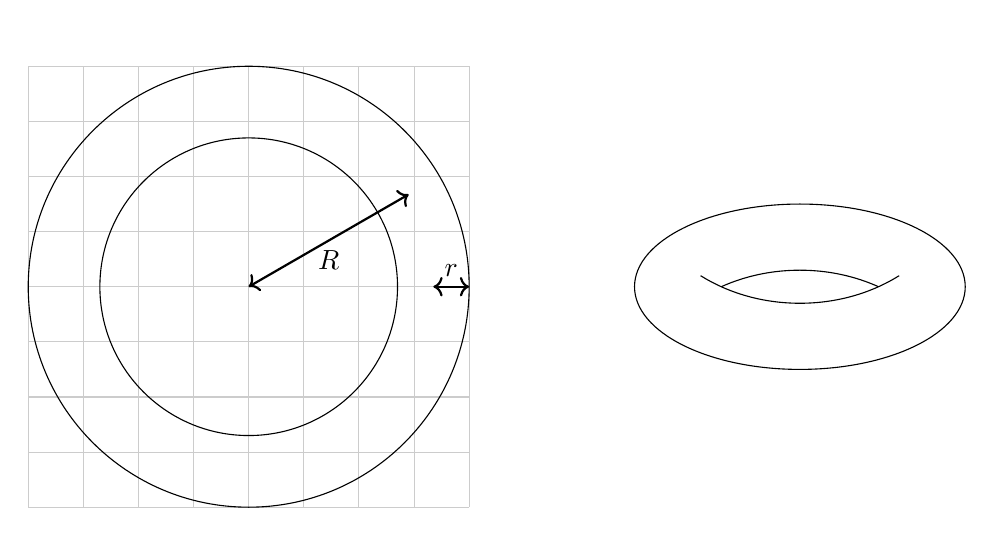
\begin{tikzpicture}[scale = 0.7]
        \draw[lightgray!80] (-4, -4) grid (4, 4);
        %\fill[double distance=5mm, fill=white, draw=black] (0:1) arc (0:180:1) (180:1) arc (180:360:1);
        \draw (0,0) circle[radius = 2.7];
        \draw (0,0) circle[radius = 4];
        \draw[<->, thick] (0, 0) -- node[below] {\(R\)} ++(30:3.35);
        \draw[<->, thick] (3.35, 0) -- node[above] {\(r\)} ++(0.65, 0);
        \draw (10,0) ellipse (3 and 1.5);
        {
            \clip (10,-1.8) ellipse (3 and 2.5);
            \draw (10,2.2) ellipse (3 and 2.5);
        }
        {
            \clip (10,2.2) ellipse (3 and 2.5);
            \draw (10,-2.2) ellipse (3 and 2.5);
        }
    \end{tikzpicture}
\end{center}

\vspace{5px}

For a sphere with parameters \(u\) and \(v\), \(r\) as the radius
\[
    \mathbf{p}: \mathbb{R}^2 \rightarrow \mathbb{R}^3
\]
\begin{align*}
    x &= r \cos(u) \cos(v)\\
    y &= r \sin(u) \cos(v)\\
    z &= r \sin(v)
\end{align*}

\[
    (u,v) \in [0,2\pi) \times [-\frac{\pi}{2}, \frac{\pi}{2}]
\]

\begin{center}
    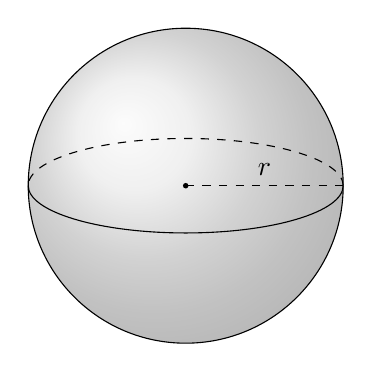
\begin{tikzpicture}
        \shade[ball color = gray!40, opacity = 0.4] (0,0) circle (2cm);
        \draw (0,0) circle (2cm);
        \draw (-2,0) arc (180:360:2 and 0.6);
        \draw[dashed] (2,0) arc (0:180:2 and 0.6);
        \fill[fill=black] (0,0) circle (1pt);
        \draw[dashed] (0,0 ) -- node[above]{\(r\)} (2,0);
    \end{tikzpicture} 
\end{center}

\newpage

\subsubsection{Bezier Curves}

A more complex case of parametric curves is a Bezier curve.

\begin{defin}[Bezier Curves]{thm:bezier-curves}
    A \textbf{Bezier Curve} is a parametric curve which has a weighted combination
    of basis functions (\(B_{i}^n\)). The weights (also called control points) are a set of points
    (\(\mathbf{p}_i\)) in 2D space.
    \begin{gather*}
        \mathbf{p}(t) = \sum_{i=0}^n \mathbf{p}_i B_i^n(t)\\
        B_i^n(t) = \binom{n}{i} t^i (1-t)^{n-i}
    \end{gather*}
\end{defin}

\vspace{10px}

\begin{center}
    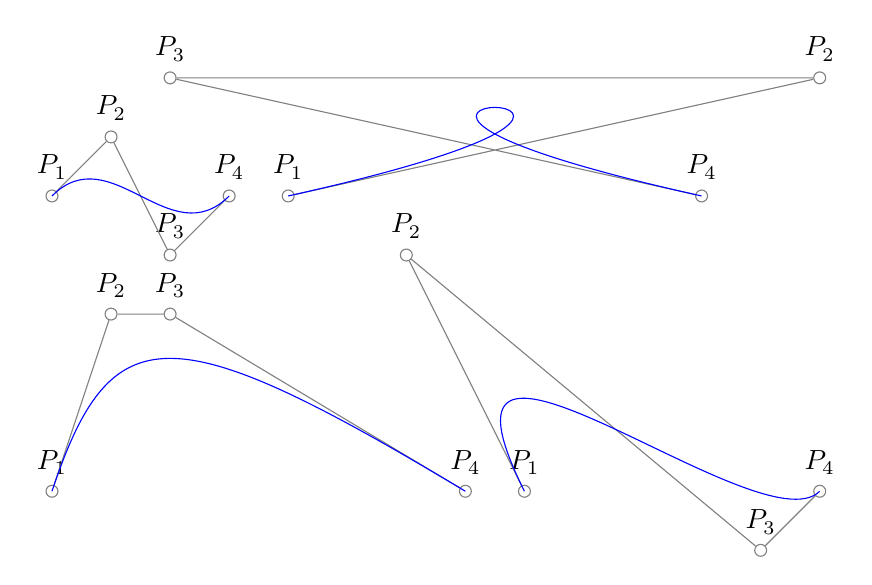
\begin{tikzpicture}[scale=0.75]
    \Bezier{0,0}{1,1}{2,-1}{3,0}
    \begin{scope}[xshift=4cm]
        \Bezier{0,0}{9,2}{-2,2}{7,0}
    \end{scope}
    \begin{scope}[yshift=-5cm]
        \Bezier{0,0}{1,3}{2,3}{7,0}
    \end{scope}
    \begin{scope}[xshift=8cm,yshift=-5cm]
        \Bezier{0,0}{-2,4}{4,-1}{5,0}
    \end{scope}
    \end{tikzpicture} 
\end{center}

\subsubsection{Bezier Surfaces}

\begin{defin}[Bezier Surfaces]{thm:bezier-surfaces}
    A \textbf{Bezier Surface} is an extension of \nameref{thm:bezier-curves} to the 3D space.
    Similarly it is a weighted combination of basis functions. The weights \(\mathbf{p}_{i,j}\) are 
    now 3 dimensional vectors and are the control points that define the control polygon.

    \vspace{10px}

    Instead of having just \(t\) varying and having \textbf{p} be a function of one variable
    we now have \(u\) and \(v\) and \(\mathbf{p}: \R^2 \to \R^3\).
    
    \vspace{5px}

    (\(B_{i}^n\) is same definition as above).

    \[
        \mathbf{p}(u,v) = \sum_{i=0}^m \sum_{j=0}^n \mathbf{p}_{i,j} B_i^m (u) B_j^n (v)
    \]
\end{defin}



\newpage

\subsubsection{Volumetric Representations}

\begin{defin}[Volumetric Representations]{thm:volumetric-representations}
    \textbf{Volumetric Representations} of geometry can be thought of as fields scalar fields in \(\mathbb{R}^{3}\)
    where each point has a value that determines a property that we are interested in for example in MRI's it
    may be the density of tissue at that point. It may also be a colour.

    \vspace{5px}

    It still follows the general form of parametric curves and surfaces with \(m=3\) and \(n=1\), but rather than
    mapping from a lower dimension to a higher dimension it is in reverse mapping from \(\mathbb{R}^{3}\) to 
    just a single real value representing the scalar quantity.
\end{defin}


\begin{center}
    \scalebox{1.5}{\(f:\, X \rightarrow Y, X \subseteq \R^3, Y \subseteq \R\)}
\end{center}
\begin{figure}[!ht]
    \centering
    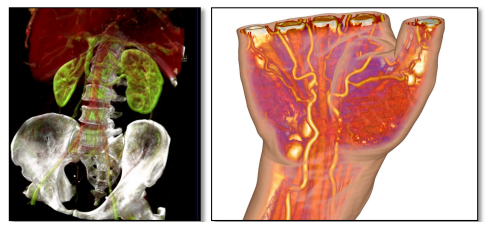
\includegraphics[width=0.75\linewidth]{images/volumetric_representations.png}
\end{figure}

\subsubsection{Parametric Curve \& Surfaces Pros and Cons}


\begin{tabular}{rl}
    + &Easy to generate points on a curve/surface\\
    + &Easy point-wise differential properties\\
    + &Easy to control by hand\\
    \minus &Hard to determine inside/outside\\
    \minus &Hard to determine if a point is on a curve/surface\\
    \minus &Hard to generate by reverse engineering\\
\end{tabular}



\newpage
\subsection{Meshes}

\begin{defin}[Meshes]{thm:meshes}
    Meshes in CG are points in 2D or 3D connected by edges forming polygons, e.g. triangles.
    They represent the boundary of an object as a discrete surface.

    \vspace{5px}
    
    A polygonal mesh is a piecewise linear approximation of an underlying continuous surface.
    As the number of polygons increases the mesh approaches the true surface. Very quickly
    which is very useful.

    A surface mesh is a graph embedded in 3D to go from a graph to a mesh we need postitions \(\mathbf{p}\)
    for each vertex.

    \vspace{10px}

    Each vertex in \(V\) is associated with a point \(p\) in 3D.

    \vspace{5px}

    The vertices are connected by edges in \(E\).

    \vspace{5px}

    The edges form faces stored in a set \(F\). 
\end{defin}

\begin{minipage}{0.7\textwidth}
    \begin{alignat*}{6}
        &V && = \{ v_1, \cdots, v_n&&\}\\
        &E && = \{ e_1, \cdots, e_k&&\}, \qquad &&e_i &&\in V \times V\\
        &F && = \{ f_1, \cdots, f_m&&\}, &&f_i &&\in V \times V \times V\\[10px]
        &P && = \{\mathbf{p}_{1}, \cdots, \mathbf{p}_{n}&&\}, &&\mathbf{p}_i &&\in \R^3\\
    \end{alignat*}
\end{minipage}
\begin{minipage}{0.25\textwidth}
    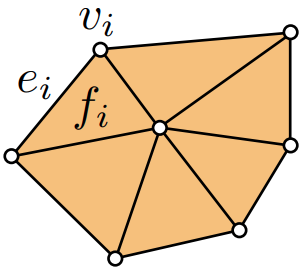
\includegraphics[width=0.9\linewidth]{images/mesh_graph.png}
\end{minipage}




\subsection{Implicit curves \& Surfaces} \label{implicit-curves/surfaces}

\begin{defin}[Implicit Objects]{thm:implicit-objects}
    \[
        f: \R^m \to \R
    \]

    Implicit objects are the set of zeroes of a function, \(m=2\) for a curve in 2D or \(m=3\) for a surface
    or curve in 3D
\end{defin}

\begin{center}
    Planar Curves 2D \hspace{50px} Surfaces in 3D

    \vspace{-10px}

    \[
        S = \{\text{\textbf{x}} \in \mathbb{R}^2 \, |\  f(\text{\textbf{x}}) = 0\} \qquad
        S = \{\text{\textbf{x}} \in \mathbb{R}^3 \, |\  f(\text{\textbf{x}}) = 0\}
    \]
\end{center}

\vspace{-10px}

\begin{figure}[!ht]
    \centering
    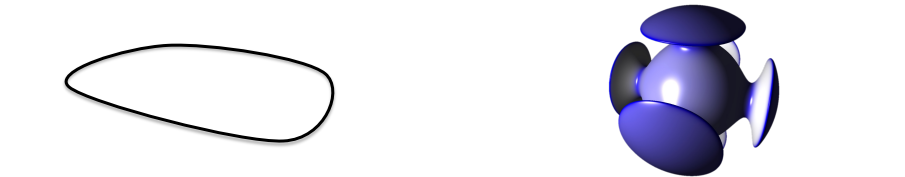
\includegraphics[width=0.5\linewidth]{images/planar_vs_surfaces.png}
\end{figure}


To define a solid object the implicit function can be extended to include the inside of the surface.

\begin{align*}
    \{ x & \in \R^m | f(x) > 0\} \qquad \text{\textcolor{red}{Outside}}\\
    \{ x & \in \R^m | f(x) = 0\} \qquad \text{The Surface/Curve}\\
    \{ x & \in \R^m | f(x) < 0\} \qquad \text{\textcolor{blue}{Inside}}\\
\end{align*}


\newpage

To shift a function to a new center that is not the origin it is as simple as:

\[
    f(\text{\textbf{x}}) \ \text{Shifted from origin to } \text{\textbf{x}}_0 \text{ is } 
    f(\text{\textbf{x}}-\text{\textbf{x}}_0)
\]


\vspace{15px}

\subsubsection{Implicit Examples}

For example for a circle centered at origin the implicit equation is  \(f(x,y) = x^2 + y^2 - r^2\) 

and for a sphere at the origin it is \(f(x,y,z) = x^2 + y^2 + z^2 - r^2\)


\vspace{10px}
The surface normal is calculated by taking the derivatives of \(f\).

\[
    \mathbf{n} = \nabla f(x,y,z) = \left(\pdv{f}{x}, \pdv{f}{y}, \pdv{f}{z}\right)^T
\]


The normal \(\mathbf{n}\) obtained is not normalised so to normalise

\[
    \hat{\mathbf{n}} = \frac{\nabla f(x,y,z)}{||\nabla f(x,y,z)||}
\]

For the case of a sphere:

\begin{align*}
    \hat{\mathbf{n}} = \frac{\nabla f(x,y,z)}{||\nabla f(x,y,z)||} &= 
    \frac{(2x, 2y, 2z)^T}{\sqrt{4x^2 + 4y^2 + 4z^2}}\\[2px]
    &= \frac{(x, y, z)^T}{\sqrt{x^2 + y^2 + z^2}}
\end{align*}


So for a sphere with radius 1 the surface normal is just the position vector.

\vspace{20px}

\subsubsection{Implicit Object Pros and Cons}

\begin{tabular}{rl}
    + &Easy to determine inside/outside\\
    + &Easy to determine if a point is on a curve/surface\\
    + &Easy to combine\\
    \minus &Hard to generate points on a curve/surface\\
    \minus &Limited set of surfaces\\
    \minus &Does not lend itself to real-time rendering\\
\end{tabular}

\newpage



\subsection{Point Set Surfaces}

One practical representation that combines some advantages of parametric and
implicit representations are point set surfaces.

A point set surface is defined in terms of a point cloud in 3D.

A point cloud is a set of points possibly with a point-wise attribute (position, surface normal, colour etc.).

The data acquired normally comes from real-world, so quite important in practice.

One particular form a point set surface is defined via locally fitting a proxy surface


\vspace{20px}
To go from a point set to an implicit function. One way is \textbf{Local Fitting}.

\subsubsection{Local Fitting}

\begin{defin}[Local Fitting]{thm:local-fitting}
    Locally just looking at any point in space the surface patch of the point set closest to the point
    can be estimated as a simple object, in 3D a plane.
\end{defin}

In the case of the curve a simple line.

\begin{figure}[!ht]
    \centering
    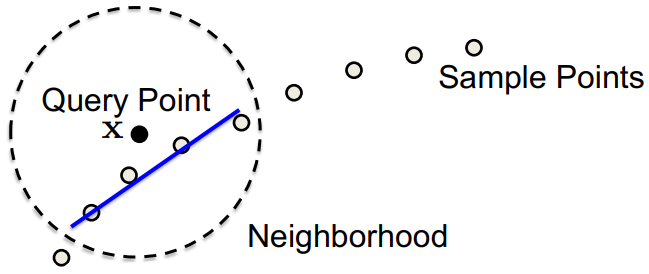
\includegraphics[width=0.5\linewidth]{images/local_fitting.png}
\end{figure}

\vspace{10px}

The distance to the surface can then be approximated with the distance to this local proxy surface.
Which is a lot faster than trying to use the point set explicitly.

\begin{figure}[!ht]
    \centering
    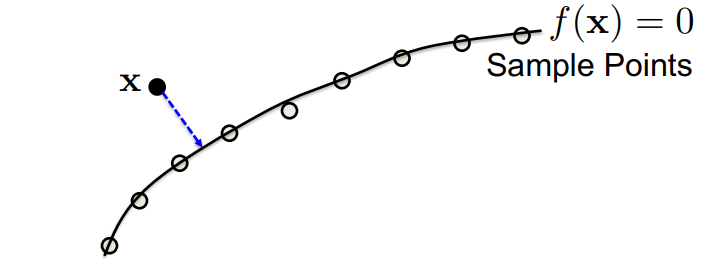
\includegraphics[width=0.5\linewidth]{images/fully_fitted.png}
\end{figure}

The local approximations combine to make a global approximation, it has \textbf{fast projection} of points 
onto the surface.
This is done by looking at the point and its nearest neighbours and project onto the local plane or line.

This means, as opposed to implicit functions, its easier to generate points on the surface
(or approximations of points on the surface)


\vspace{30px}

\subsubsection{Point Set Surfaces Pros and Cons}

\begin{tabular}{rl}
    + &Easy to determine inside/outside\\
    + &Easy to determine if a point is on a curve/surface\\
    + &Easy to generate points on the curve/surface\\
    + &Suitable for reconstruction from general data\\
    + &Direct real-time rendering (although not as fast as triangle meshes)\\
    + &Easily converted to a triangle mesh\\
    + &Robust to noise\\
    \minus &Not efficient to use in some modelling tasks
\end{tabular}


\newpage

\section{Discrete Differential Geometry}
\subsection{Manifolds}

\begin{defin}[Open-Surfaces]{thm:open-surfaces}
    An \textbf{Open Ball} of radius \(r\) and center \(\mathbf{x}\) is the set of all points \(\mathbf{p}\) 
    such that they are a distance \textbf{less than} \(r\) away from \(\text{\textbf{x}}\)
    
    \[
        |\mathbf{x}-\mathbf{p}| < r
    \]
    
    Similarly an \textbf{Open Disk} of radius \(R\) and center \(\mathbf{x}\) is the set of all points on 
    the plane at a distance \textbf{less than} \(R\) from \(\mathbf{x}\).
\end{defin}

\begin{defin}[Manifolds]{thm:Manifolds}
    A \textbf{Surface} is a \textbf{Closed 2-Manifold} if it is locally homeomorphic to a disk everywhere.

    \vspace{5px}

    \textit{(More formally)}

    For every point \(\mathbf{x}\) in \(M\), there is an \hyperref[thm:open-surfaces]{\textbf{Open Ball}}
    \(B_{x}(r)\) of radius \(r\) centred at \(\mathbf{x}\) such that \(M \cap B_{x}(r)\)
    is homeomorphic to an open disk.

    \vspace{10px}

    \textit{(Less formally)}

    Locally everywhere on the surface is a plane.
\end{defin}

\begin{figure}[!ht]
    \centering
    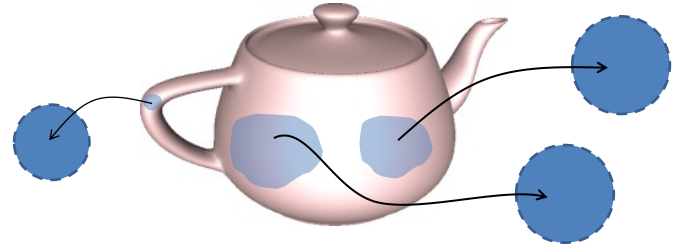
\includegraphics[width=0.5\linewidth]{images/2-manifold.png}
\end{figure}

\subsubsection{Manifolds with Boundaries}
\vspace{10px}
\begin{defin}[Manifolds With Boundaries]{thm:Manifolds-with-boundaries}
    If all points at boundaries are homeomorphic to a half-disk (semi-circle), and points not at boundaries obey
    the 2-manifold principle of being homeomorphic to an open disk locally then that surface is a manifold with
    boundaries.
\end{defin}

\begin{figure}[!ht]
    \centering
    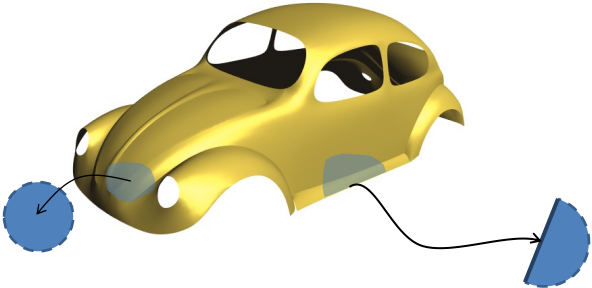
\includegraphics[width=0.5\linewidth]{images/manifold_with_boundaries.png}
\end{figure}

Having these properties allows for differential geometry.

\newpage
\subsection{Differential Geometry Properties}

For every point on the surface you can define  a local parameter space, which is local parametric
representation of the surface. And this always works for manifolds. Similar to Parametric Surfaces
but just locally.

\vspace{5px}

Having the local parametric representation allows us to do partial derivatives with respect to \(u\) and \(v\)
to obtain normals and other useful stuff.

\begin{figure}[!ht]
    \centering
    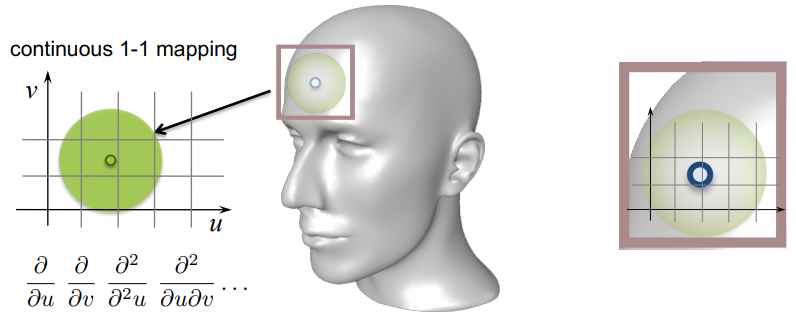
\includegraphics[width=0.6\linewidth]{images/local_observations.png}
\end{figure}


\subsubsection{Local Coordinates}

To define local coordinates we have a surface patch and locally its a disk, and from the manifold properties we
can define a \(u\)-\(v\) domain and from the parametric surfaces before we can define a function 
\(\mathbf{p}(u,v)\) mapping from the \(u\)-\(v\) to points on the surface.

\begin{figure}[!ht]
    \centering
    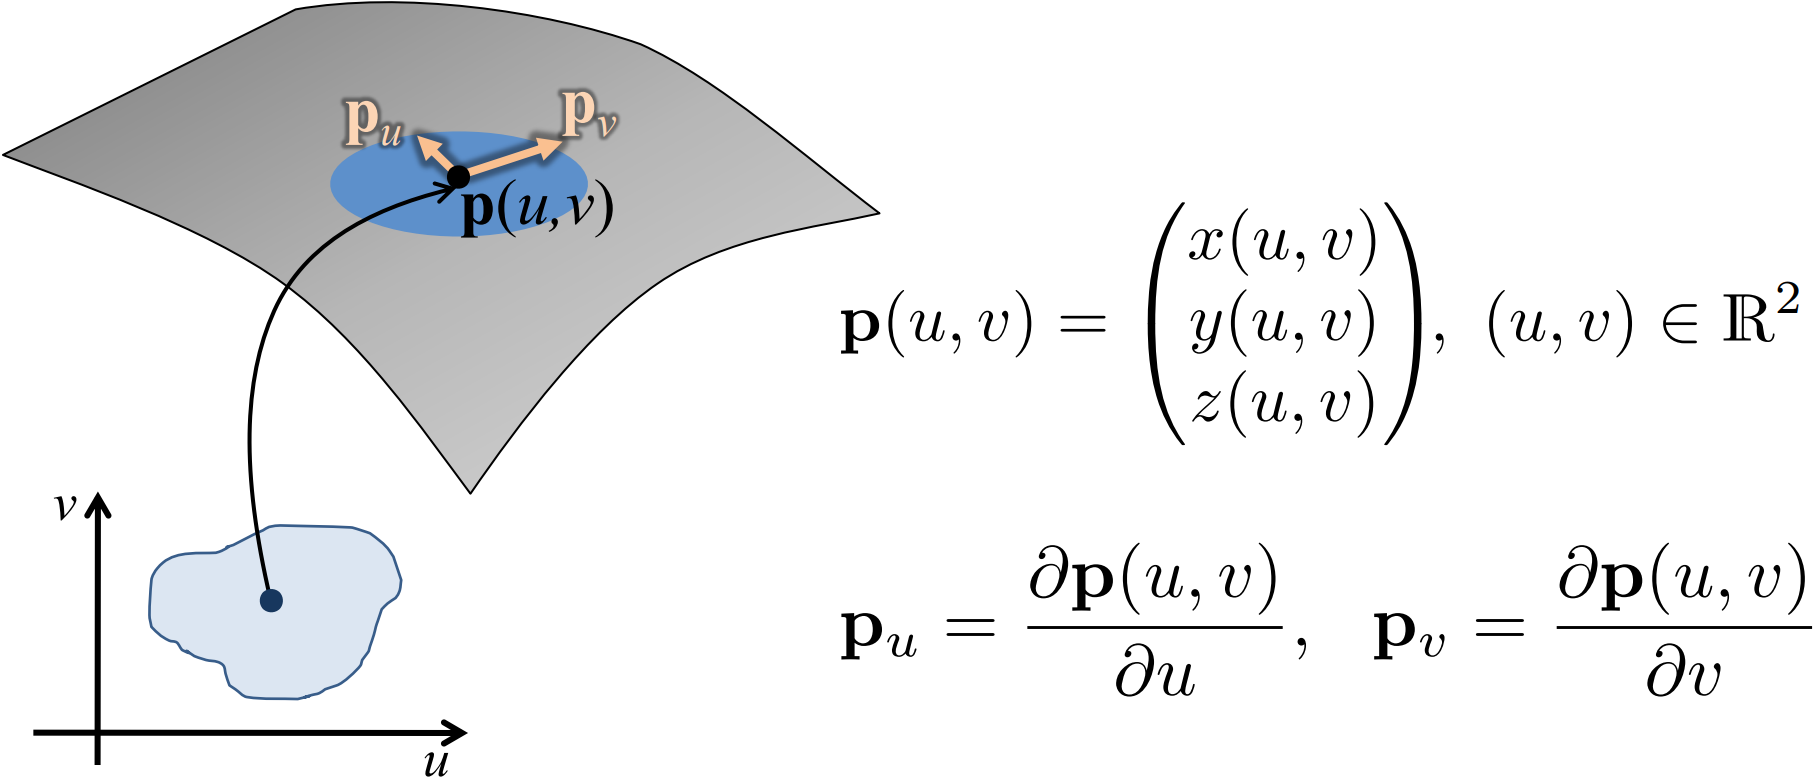
\includegraphics[width=0.7\linewidth]{images/local_coords.png}
\end{figure}


Like seen in Parametric Surfaces \(\mathbf{n}\) can be obtained with these two vectors \(\mathbf{p}_{u}\) and
\(\mathbf{p}_{v}\)

\[
    \mathbf{p}_{u} \times \mathbf{p}_{v} \neq \mathbf{0}\\
\]

\[
    \mathbf{\hat{n}}(u,v) = \frac{\mathbf{p}_{u} \times \mathbf{p}_{v}}
    {||\mathbf{p}_{u} \times \mathbf{p}_{v}||}
\]

\newpage
\subsubsection{Normal Curvature}

\begin{figure}[!ht]
    \centering
    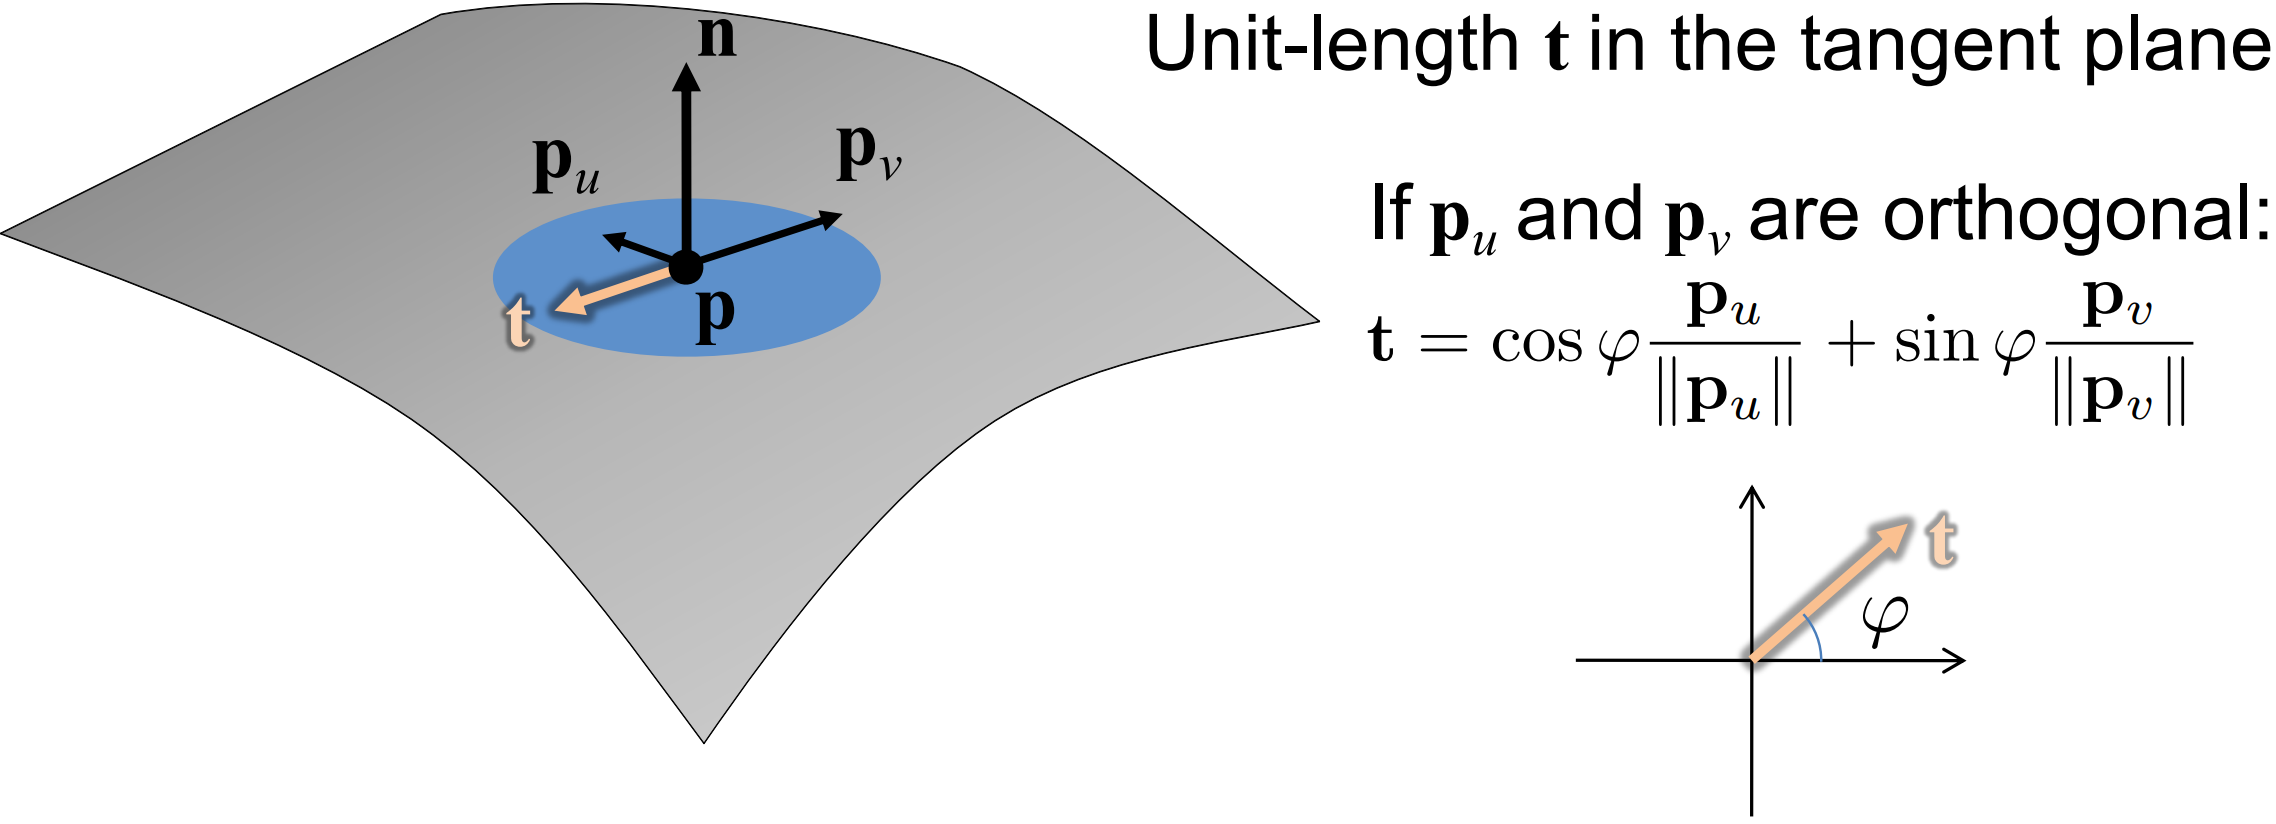
\includegraphics[width=0.6\linewidth]{images/curvature_1.png}
\end{figure}

\(\mathbf{p}_u\) and \(\mathbf{p}_v\) are basis vectors so any point on the local disk can be represented
as a linear combination of the two.

As \(\varphi\) varies the \(\mathbf{t}\) rotates around \(\mathbf{n}\) in the tangent plane. For each of these
rotated \(\mathbf{t}\)'s there is a different curvature.


\begin{figure}[!ht]
    \centering
    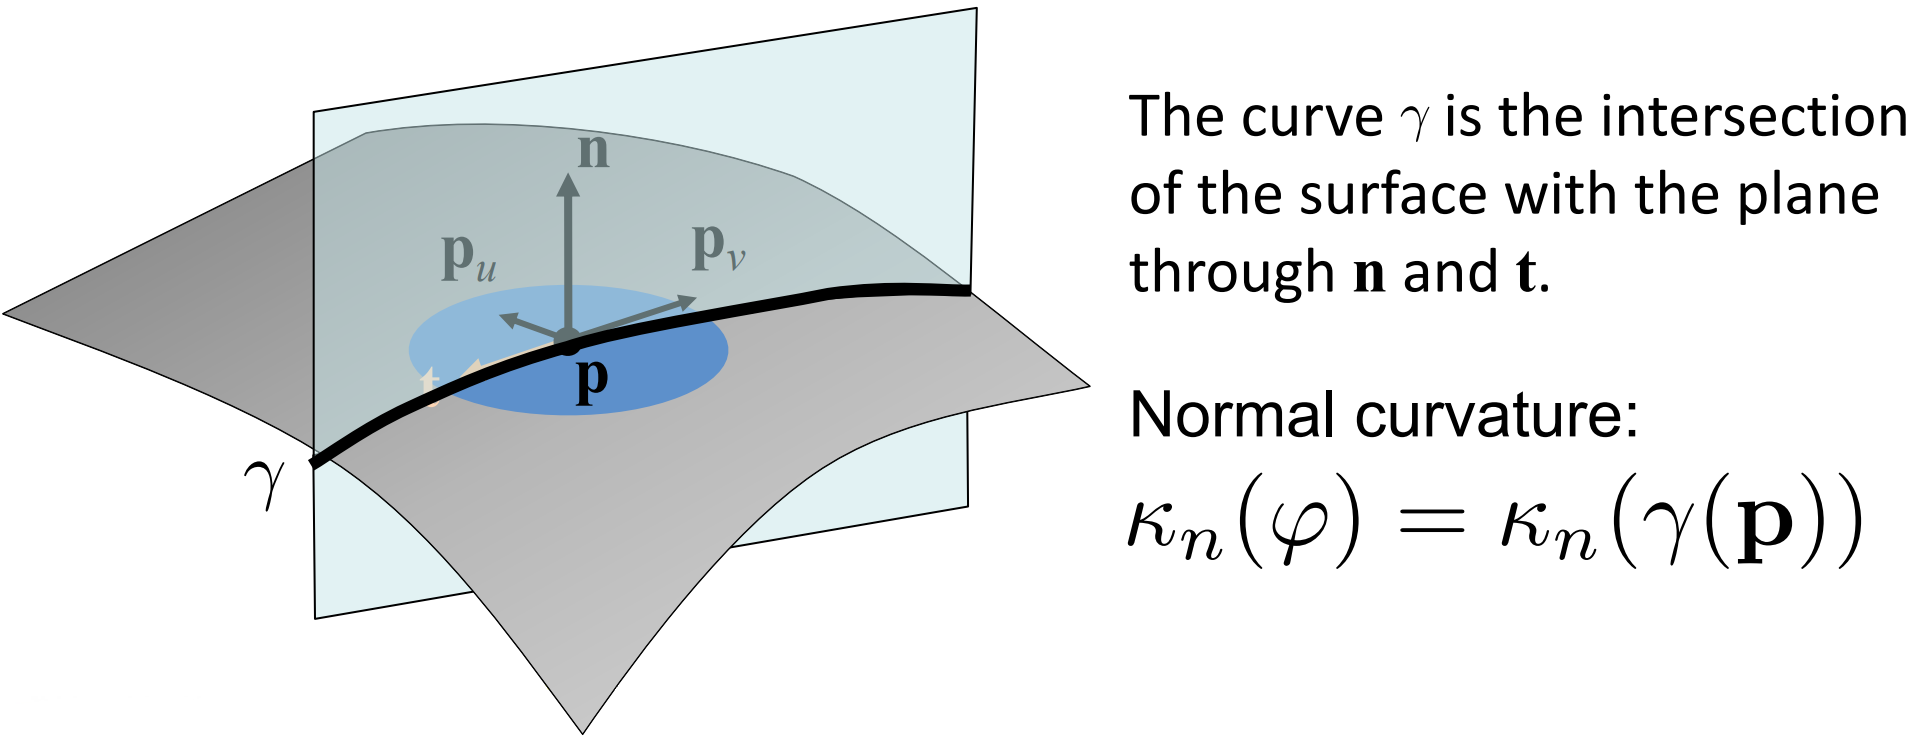
\includegraphics[width=0.6\linewidth]{images/curvature_2.png}
\end{figure}

\subsubsection{Planar Curves (New stuff this year)}

Looking at the the intersection we get a planar curve for each direction.

\vspace{5px}

Like seen previously they can be paramterised by a single paramter \(t\).

\[
    \mathbf{p}(t) = \begin{pmatrix}
        x(t)\\
        y(t)
    \end{pmatrix}\, , \ t \in [t_{0}, t_{1}]
\]

\begin{figure}[!ht]
    \centering
    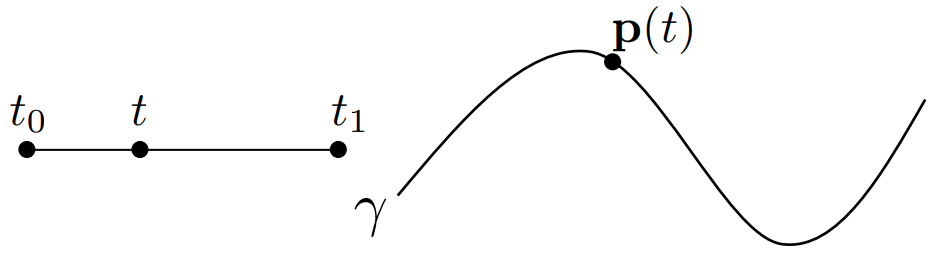
\includegraphics[width=0.5\linewidth]{images/planar_curvature.png}
\end{figure}

A given curve can have infinitely many paramerisations.

\vspace{5px}

Imagine walking along the curve the speed of the walk can change at any point from one end to the other.

\vspace{5px}

We choose a specific paramerisation, where the absolute value of the derivative w.r.t. \(t\) is a constant.

\[
    \lVert \frac{\partial \mathbf{p}(t)}{\partial t} \rVert = 1 
\]

With such a so-called arc-length parametrisation, we can define the tangent vector, 
normal vector, and curvature in terms of the first and second derivatives of the curve with simplified forms.

\begin{minipage}{0.435\textwidth}
    \[
        \mathbf{t} = \frac{\partial \mathbf{p}(t)}{\partial t}
    \]
    \[
        \frac{\partial^2 \mathbf{p}(t)}{\partial t^2} = \kappa(t) \mathbf{n}(t)
    \]
\end{minipage}
\begin{minipage}{0.435\textwidth}
    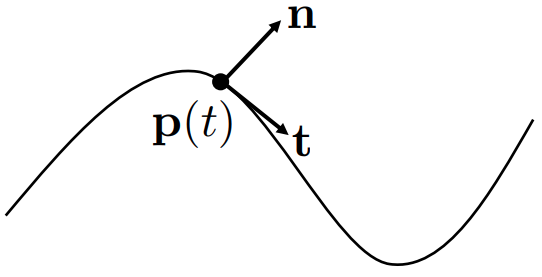
\includegraphics[width=0.7\linewidth]{images/planar_tang_norm.png}
\end{minipage}






\newpage

\begin{defin}[Osculating/Best-Fitting Circle]{thm:osculating}
    An \textbf{Osculating Circle} is a circle with radius equal to the inverse of the absolute value of the
    curvature at the point \(\mathbf{p}\).

    \vspace{5px}

    Its essentially the circle that best approximates the region around \(\mathbf{p}\).
\end{defin}

\begin{figure}[!ht]
    \centering
    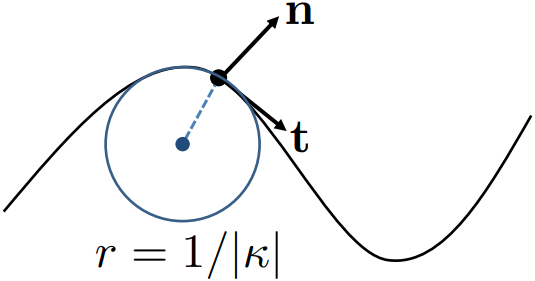
\includegraphics[width=0.4\linewidth]{images/osculating_circle.png}
\end{figure}


The best way to approximate this \textbf{Osculating} circle for a parametric curve is to have two points 
either side of \(\mathbf{p}\), then when this points converge to \(\mathbf{p}\) then the circle
defined by the 3 points is the best fittting circle at \(\mathbf{p}\).

\[
    \text{The circle defined by: } \quad \lim_{\epsilon \to 0^+} \mathbf{p}(t-\epsilon), \mathbf{p}(t), \mathbf{p}(t+\epsilon) 
\]


\begin{figure}[!ht]
    \centering
    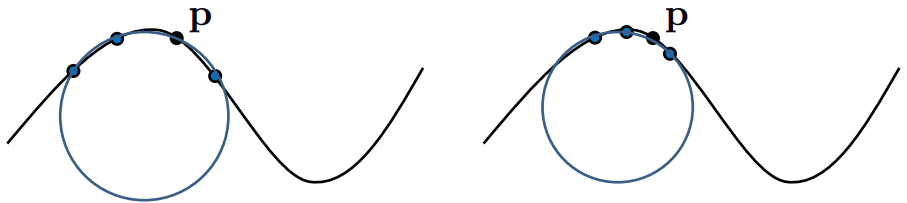
\includegraphics[width=0.8\linewidth]{images/approx_osculating_circle.png}
\end{figure}

\begin{center}
    \begin{minipage}{0.8\textwidth}
        \url{https://www.desmos.com/calculator/qd0bayp351}
        
        Desmos playground for curvature, osculating circles, tangents and normals.
    \end{minipage}
\end{center}


\begin{defin}[Principal Curvatures]{thm:principal-curvature}
    The two \textbf{Principal Curvatures} are the minimum and maximum curvatures at a point on a surface. The 
    minimum and maximum are defined below.
\end{defin}


\begin{defin}[Surface Curvatures]{thm:surface-curvatures}
    \begin{alignat*}{4}
        &\text{Minimal Curvature} \qquad &\kappa_{1} =& \ \kappa_{\text{min}} &&= \underset{\varphi}{\operatorname{min}} \, \kappa_{n}(\varphi)\\
        &\text{Maximal Curvature} \qquad &\kappa_{2} =& \ \kappa_{\text{max}} &&= \underset{\varphi}{\operatorname{max}} \, \kappa_{n}(\varphi)\\
        &\text{Mean Curvature} &H =& \ \frac{\kappa_{1} + \kappa_{2}}{2} &&= \frac{1}{2\pi} \int_{0}^{2\pi} \kappa_{n}(\varphi) \operatorname{d\varphi}\\
        &\text{Gaussian Curvature} &K =& \ \kappa_{1} \cdot \kappa_{2}
    \end{alignat*}
\end{defin}


\newpage

\begin{theo}[Euler's Theorem]{thm:euler-theorem}
    \textbf{Planes} of principal curvature are \textbf{orthogonal} and independent of parameterization.

    \begin{align*}
        \kappa_{n}(\varphi) &= \kappa_{1}\cos^2 \varphi + \kappa_{2} \sin^2 \varphi\\
        \varphi &= \text{angle with} \ \mathbf{t}_{1}
    \end{align*}
\end{theo}

Euler's Theorem says that we can write any curvature as a linear combination of the principal curvatures. 
\(\varphi\) is the angle between the direction for the curvature and that for minimum normal curvature.


\begin{figure}[!ht]
    \centering
    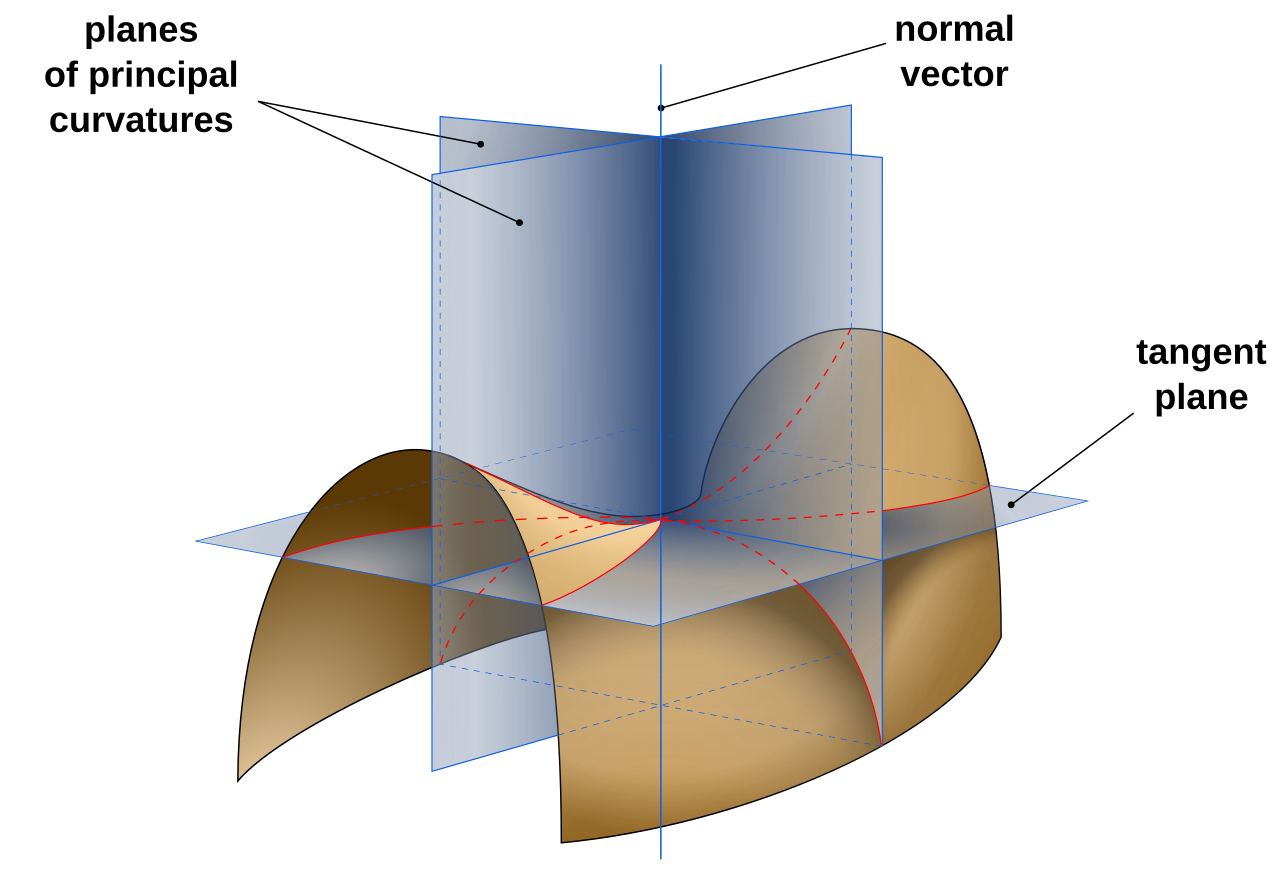
\includegraphics[width=0.5\linewidth]{images/principal_curvature.png}
\end{figure}

\begin{prf}[Mean Curvature]{thm:mean-curvature}
    \begin{alignat*}{1}
        H &= \frac{1}{2\pi} \int_{0}^{2\pi} \kappa_{n}(\varphi) \operatorname{d\varphi}\\
          &= \frac{1}{2\pi} \int_{0}^{2\pi} \kappa_{1}\cos^2(\varphi) + \kappa_{2} \sin^2 (\varphi) \operatorname{d\varphi}\\
          &= \frac{1}{2\pi} \int_{0}^{2\pi} \kappa_{1}(1-\sin^2(\varphi)) + \kappa_{2} \sin^2 (\varphi) \operatorname{d\varphi}\\
          &= \frac{1}{2\pi} \int_{0}^{2\pi} \kappa_{1} + (\kappa_{2}-\kappa_{1}) \sin^2 (\varphi) \operatorname{d\varphi}\\
          &= \kappa_{1} + \frac{1}{2\pi} \int_{0}^{2\pi} (\kappa_{2}-\kappa_{1}) \sin^2 (\varphi) \operatorname{d\varphi}\\
          &= \kappa_{1} + \frac{1}{2\pi} \int_{0}^{2\pi} \frac{1}{2}(\kappa_{2}-\kappa_{1}) (1- \cos(2\varphi)) \operatorname{d\varphi}\\
          &= \kappa_{1} + \frac{1}{2}(\kappa_{2}-\kappa_{1}) + \frac{1}{2\pi} \int_{0}^{2\pi} - \cos(2\varphi) \operatorname{d\varphi}\\
          & = \frac{\kappa_{1} + \kappa_{2}}{2}
    \end{alignat*}
    
\end{prf}


\newpage

\begin{defin}[Isotropic Shapes]{thm:isotropic-shapes}
    \textbf{Isotropic} means all directions are principal directions.

    \vspace{5px}

    Shapes with an \hyperref[thm:surface-curvatures]{Gaussian Curvature} \(K > 0, \ \kappa_{1} = \kappa_{2}\)
    are spherical (umbilical). If \(K = 0\) then the surface is planar.
\end{defin}

\begin{figure}[!ht]
    \centering
    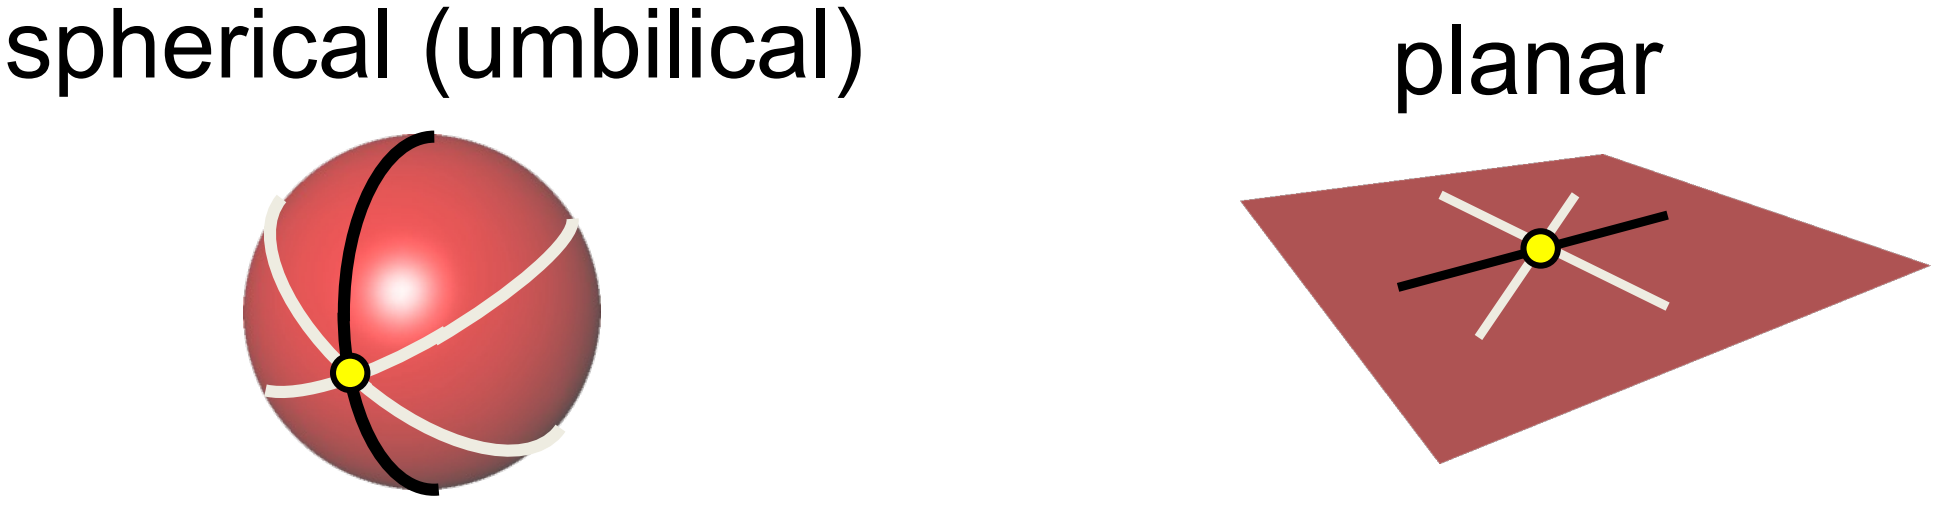
\includegraphics[width=0.5\linewidth]{images/Isotropic_Shapes.png}
\end{figure}


\begin{defin}[Anisotropic]{thm:anisotropic-shapes}
    \textbf{Anisotropic} means that there are 2 distance principal directions at any point on the surface

    \vspace{5px}

    If \(K > 0\) then the shape is elliptic

    If \(K = 0\) then the shape is parabolic

    If \(K < 0\) then the shape is hyperbolic
\end{defin}

\begin{figure}[!ht]
    \centering
    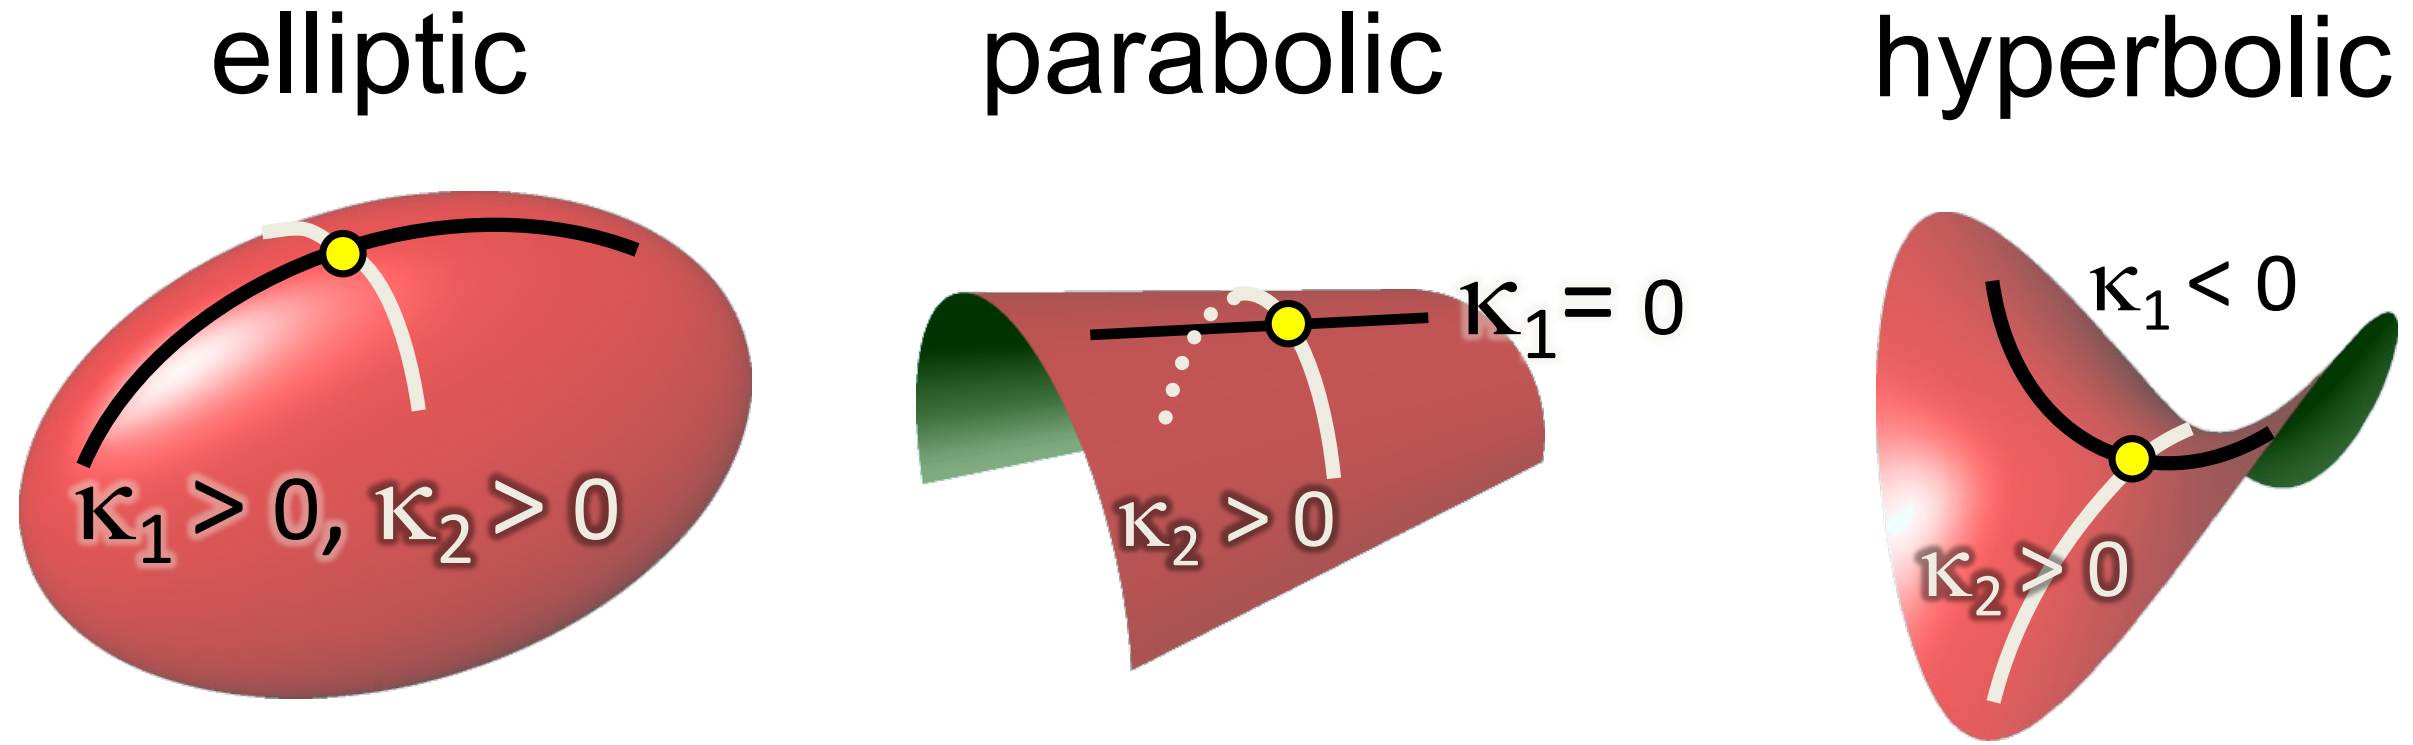
\includegraphics[width=0.5\linewidth]{images/Anistropic_Shapes.png}
\end{figure}

\newpage

\subsubsection{Laplace-Beltrami}

\begin{defin}[Laplace Operator]{thm:laplace-operator}
    Also known as the Laplacian.
    \[
        f\!\!: \, \R^{3} \to \R \qquad \Delta f\!\!: \, \R^{3} \to \R
    \]

    \[
        \Delta f = \operatorname*{div} \nabla f = \frac{\partial^2 f}{\partial x^2} + \frac{\partial^2 f}{\partial y^2} + \frac{\partial^2 f}{\partial z^2}
    \]
\end{defin}

This sum of second order derivatives is due to the following:

\[
    \operatorname{grad} f = \nabla f = \left( \frac{\partial f}{\partial x}, \frac{\partial f}{\partial y}, \frac{\partial f}{\partial z} \right)
\]

\[
    \operatorname*{div} \mathbf{F} = \nabla \cdot \mathbf{F} = \pdv{F_{x}}{x} + \pdv{F_{y}}{y} + \pdv{F_{z}}{z}
\]

This Laplace operator can be extended to manifold surfaces. Lets assume there's a function that lives on the
surface, which is not a Euclidean space in general. We then have the same operators defined slightly differently.

This is a generalization of the Laplace operator and is called the Laplace-Beltrami operator.


\begin{defin}[Laplace-Beltrami Operator]{thm:laplace-beltrami-operator}
    \begin{align*}
        f\!\!:& \ \mathcal{M} \to \R\\
        \Delta f\!\!:& \ \mathcal{M} \to \R\\[10px]
        \Delta_{\mathcal{M}} f =& \operatorname{div}_{\mathcal{M}} \nabla_{\mathcal{M}} f
    \end{align*}

    \(\Delta_{\mathcal{M}}\) is the \textbf{Laplace-Beltrami operator}.
    \(f\) is a function on surface \(\mathcal{M}\).
\end{defin}


An interesting property of the operator is if you apply it to the coordinate function (i.e. \(f(x,y,z) = x\))
of a point on the surface. You get the scaled surface normal at that point. The scaling is exactly
\(-2\) times the mean curvature.

\begin{align*}
    \Delta_{\mathcal{M}} \mathbf{p} &= \operatorname{div}_{\mathcal{M}} \nabla_{\mathcal{M}} \mathbf{p} = -2H \mathbf{\hat{n}} \in \mathbb{R}^{3}\\
    \Delta_{\mathcal{M}} \mathbf{p} &= -2H \mathbf{\hat{n}}
\end{align*}


This operator is so important due this property as it allows us to define curvature and normal in terms of 
the the application of the operator to the coordinate function. If we can define the application to the
coordinate functions on a discrete surface, we can get the mean curvature and surface normal


\newpage
\subsection{Discrete Laplace-Beltrami}

\[
    \Delta_{\mathcal{M}} \mathbf{p} = -2H \mathbf{\hat{n}}
\]

\begin{figure}[!ht]
    \centering
    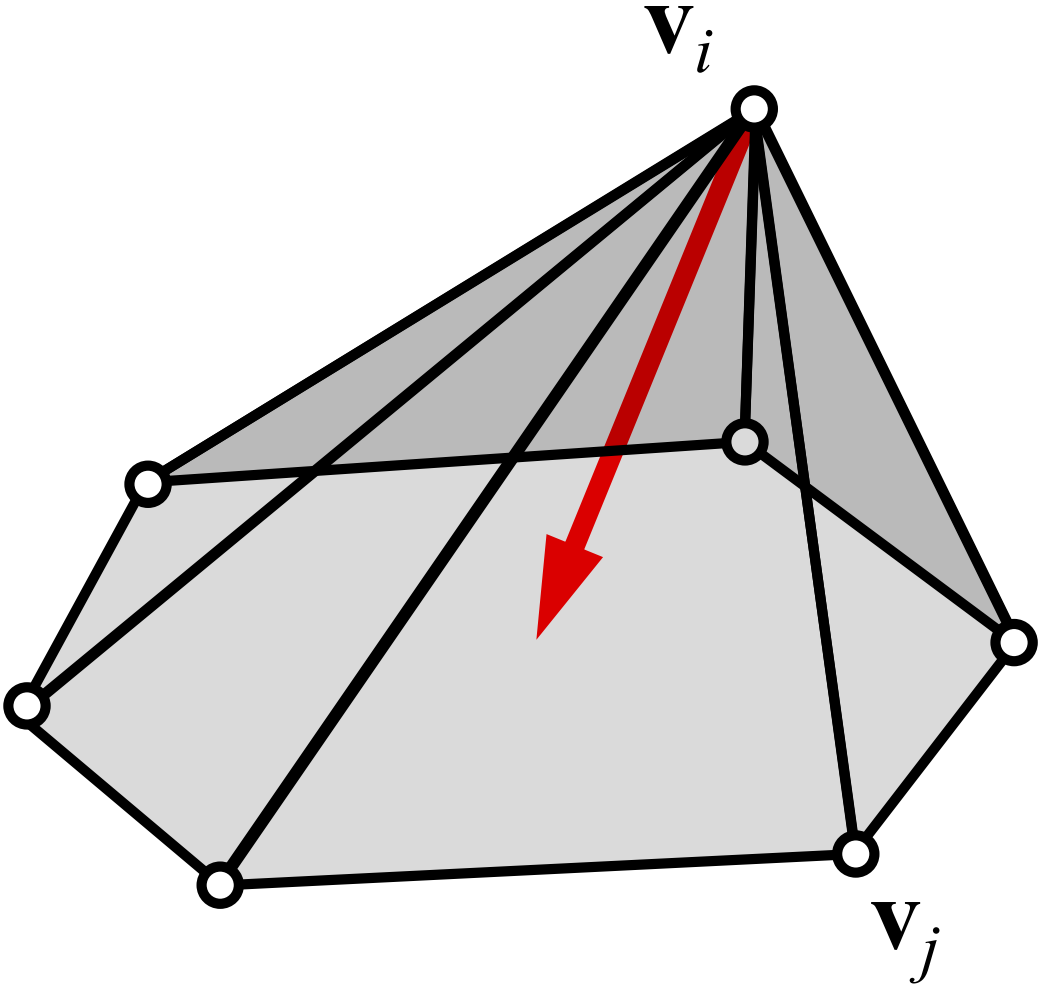
\includegraphics[width=0.2\linewidth]{images/dlb_mesh.png}
\end{figure}


We want to take the Laplace-Beltrami at the point \(\mathbf{v}_{i}\), to do this we take the average of its
connected neighbours location to get an approximation of the result and in turn an approximation of the mean
curvature and surface normal.

\begin{align*}
    L_{u}(\mathbf{v}_{i}) &= \frac{1}{|\mathcal{N}(i)|} \sum_{j \in \mathcal{N}(i)} \, (\mathbf{v}_{j} - \mathbf{v}_{i})\\
    &= \left(\frac{1}{|\mathcal{N}(i)|} \sum_{j \in \mathcal{N}(i)} \, \mathbf{v}_{j} \right) - \mathbf{v}_{i}
\end{align*}

The direction will be an approximation of the negative normal \(-\mathbf{\hat{n}}\) and the length will be \(\approx 2H\) 

\vspace{5px}

To get a closer approximation of the mean curvature and surface normal the directions can be weighted.

One general scheme for triangular meshes is using cotangent weights.

\[
    L_{c}(\mathbf{v}_{i}) = \frac{1}{A_{i}} \sum_{j \in \mathcal{N}(i)} \, \frac{1}{2} (\cot \alpha_{ij} + \cot \beta_{ij}) (\mathbf{v}_{j} - \mathbf{v}_{i})
\]

\begin{figure}[!ht]
    \centering
    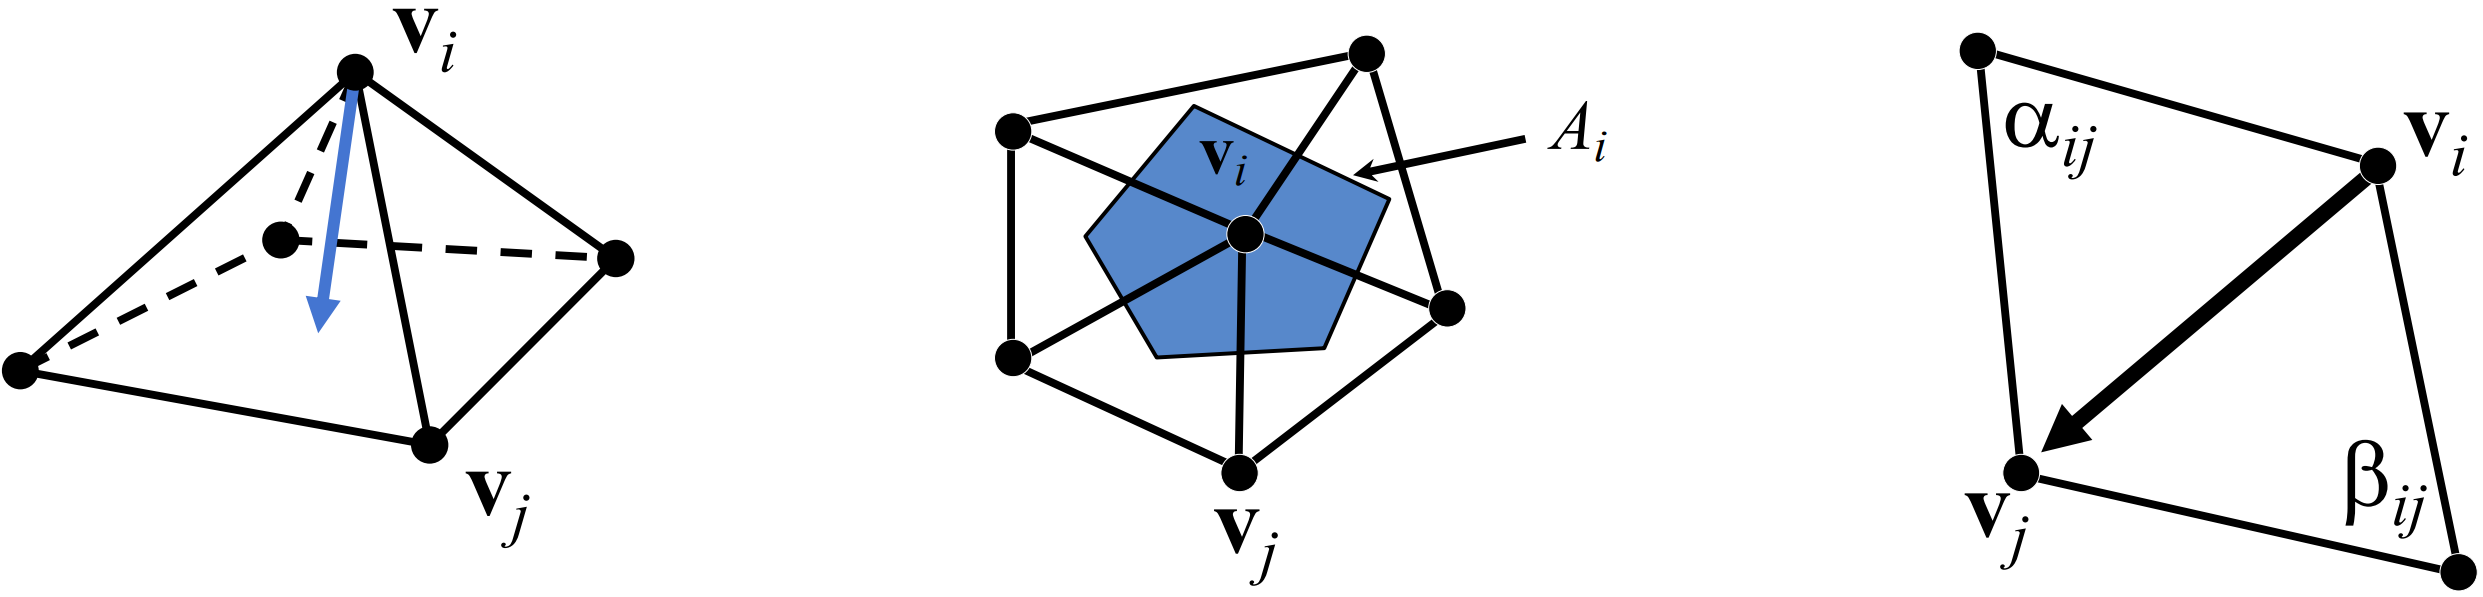
\includegraphics[width=0.7\linewidth]{images/cotangent_weighting.png}
\end{figure}

\begin{align*}
    \mathbf{c}_{j} &= 
    \begin{cases}
        \text{Circumcentre of } \triangle (\mathbf{v}_{i}, \mathbf{v}_{j}, \mathbf{v}_{j+1}) & \text{if  } \theta < \frac{\pi}{2}\\
        \text{Midpoint of edge } (\mathbf{v}_{j}, \mathbf{v}_{j+1}) & \text{if  } \theta \geq \frac{\pi}{2}
    \end{cases}\\[5px]
    A_{i} &= \sum_{j} \text{Area } (\triangle (\mathbf{v}_{i}, \mathbf{c}_{j}, \mathbf{c}_{j+1}))
\end{align*}

\begin{figure}[!ht]
    \centering
    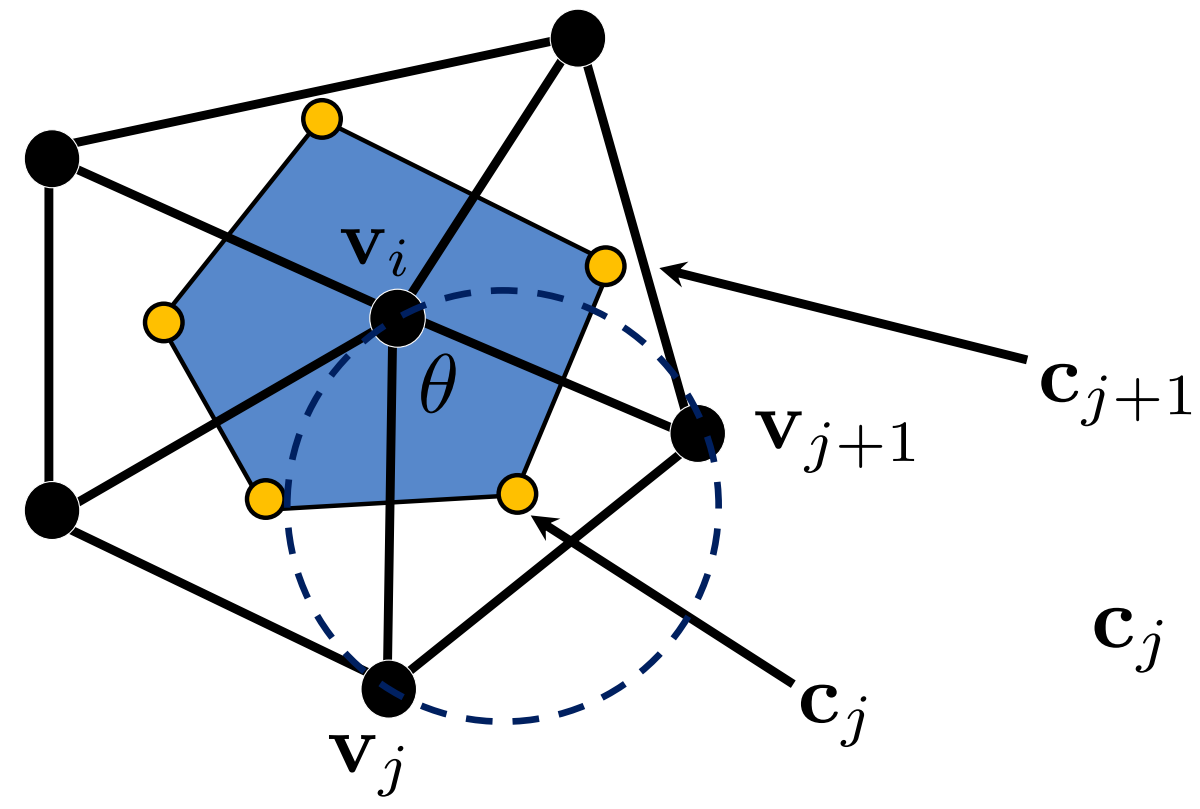
\includegraphics[width=0.3\linewidth]{images/cotangent_weights_area.png}
\end{figure}

\newpage

\subsubsection{Discrete Laplace-Beltrami Relation to Normal \& Curvature}

\begin{defin}[Discrete Laplace-Beltrami Formulas]{thm:dlp-formulas}
    \textbf{Mean Curvature} (Sign according to normal)
    \[
        |H(\mathbf{v}_{i})| = ||L_{c}(\mathbf{v}_{i})||/2
    \]

    \textbf{Gaussian Curvature}
    \[
        K(\mathbf{v}_{i}) = \frac{1}{A_{i}} \left(2\pi - \sum_{j} \theta_{j}\right)
    \]

    \textbf{Principal Curvatures}
    \vspace{5px}
    \[
        \kappa_{1} = H - \sqrt{H^{2} - K} \qquad \kappa_{2} = H + \sqrt{H^{2}-K}
    \]
\end{defin}

\begin{prf}[Principal Curvature Formulas]{thm:principal-curvature}
    Using the facts \(H = \dfrac{\kappa_1+\kappa_2}{2}\) and \(K=\kappa_1 \kappa_2 \implies \kappa_2 = \dfrac{K}{\kappa_1}\)

    \begin{alignat*}{2}
        &\phantom{\implies} &&2H = \kappa_{1} + \kappa_{2}\\
        &\implies &&2H = \kappa_{1} + \frac{K}{k_1}\\
        &\implies &&2H\kappa_{1} = \kappa_{1}^2+K\\
        &\implies &&(k_{1}-H)^2 = H^2 -K\\
        &\implies &&\kappa_{1} = H \pm \sqrt{H^2 - K} \hspace{50px} \text{Similarly } \kappa_{2} = H \pm \sqrt{H^2 - K}
    \end{alignat*}

    Since \(\kappa_{1} \leq \kappa_{2}\)

    \[
        \kappa_{1} = H - \sqrt{H^2 - K} \hspace{50px} \kappa_{2} = H + \sqrt{H^2 - K} \qquad \square
    \]
    
\end{prf}

\vspace{10px}

By considering meshes as a discrete surface we could get an approximation of the Laplace-Beltrami operator.
By doing the same for graphs or point clouds we can define an approximation of the application of the Laplace-
Beltrami operator to the coordinate function and approximate the curvatures.

In this case, the approximation is with Gaussian weights instead of Cotangent weights.

\vspace{10px}

\begin{minipage}{0.435\textwidth}
    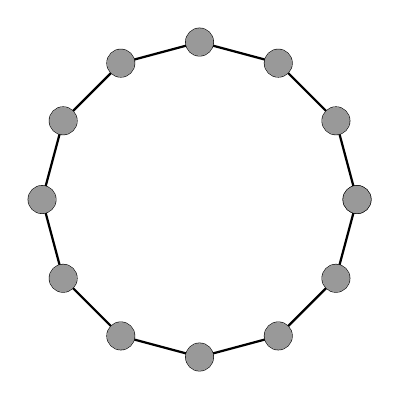
\begin{tikzpicture}
        \def \number {12}
        \def \radius {2cm}
        \def \degree {360/\number}
        
        \foreach \s in {1,...,\number}
        {
            \draw[thick] ({\degree * (\s -1)}:\radius) -- ({\degree * (\s)}:\radius);
            \draw ({\degree * (\s -1)}:\radius) circle[radius=5pt];
            \fill[black!40] ({\degree * (\s -1)}:\radius) circle[radius=5pt];
        }
        \draw ({0}:\radius) circle[radius=5pt];
        \fill[black!40] ({0}:\radius) circle[radius=5pt];
    \end{tikzpicture}
\end{minipage}
\hspace{-20px}\begin{minipage}{0.435\textwidth}
    \begin{align*}
        h_{t}(x_{i},x_{j}) &= e^{-d(x_{i}, x_{j}) / t}\\
        &= e^{-||\mathrm{\mathbf{x}}_i - \mathrm{\mathbf{x}}_j||^2 / t}
    \end{align*}

    \[
        L_{g}(x_{i}) = \frac{1}{\sum_{j=1}^n h_{t}(x_{i},x_{j})} \sum_{j=1}^{n} h_{t}(x_{i},x_{j}) (x_{j} - x_{i})
    \]
\end{minipage}

\vspace{10px}
This approximation allows us to capture complex domains, in fact any domain that can be point sampled.


\newpage
\section{Geometry Processing}

\subsection{Shape Acquisition}

\begin{figure}[!ht]
    \centering
    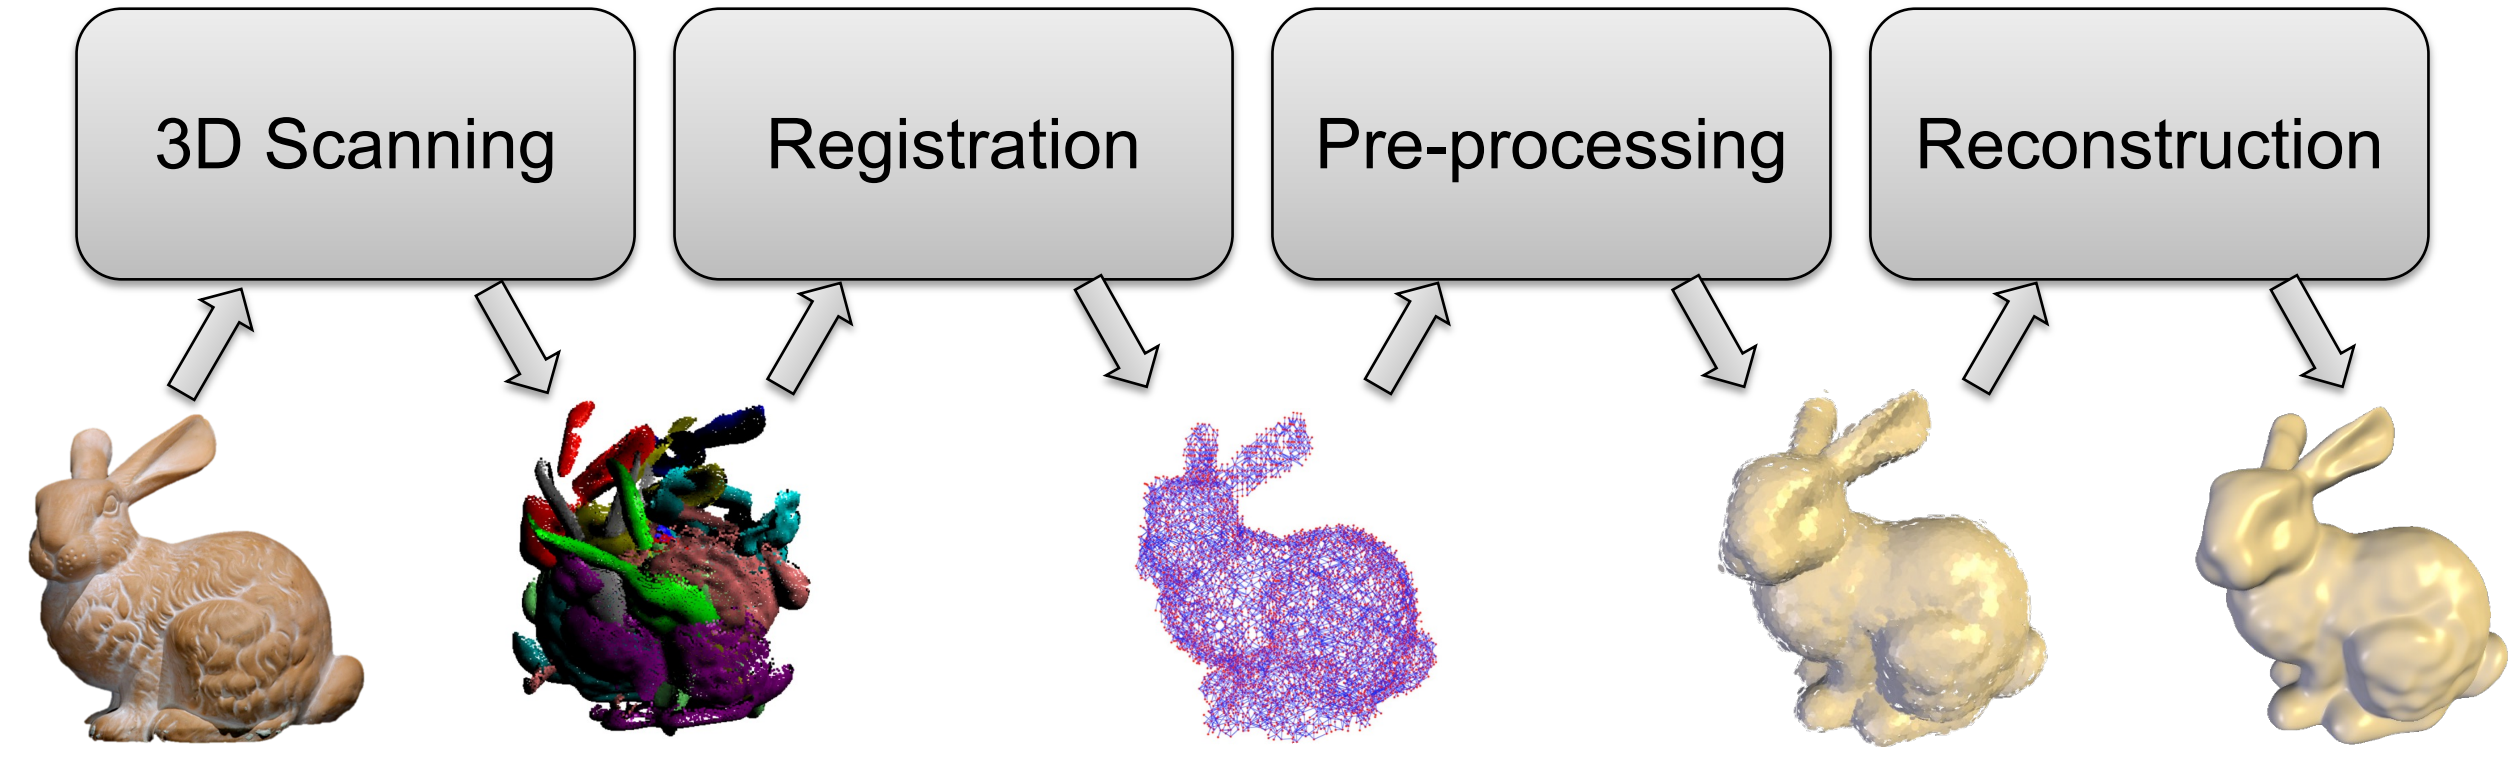
\includegraphics[width=0.8\linewidth]{images/digitization.png}
\end{figure}

It starts with \textbf{3D scanning} with a depth camera or other camera. Going from a real object to a 3D scan
and each scan is a 3D point cloud (shown in different colours)

\vspace{5px}

Then \textbf{Registration} means aligning these point clouds into a common coordinate frame so they make
a coherent point cloud of the object.

\vspace{5px}

Then \textbf{Pre-Processing} is cleaning up the point cloud so it is nicer to work with later. This could be 
reducing the number of points or removing noise from the scans.

\vspace{5px}

Then \textbf{Reconstruction} from the point cloud to create a mathematical representation of the object which can then 
be formed into a mesh.

\vspace{10px}

\subsubsection{3D Scanning}

\vspace{5px}

\textbf{Touch Probes} can be used to capture 3D objects, they are \textbf{precise} in capturing the large details of the object
However they \textbf{cannot accurately capture small objects} or fine detail on large objects, and shapes with cavities.
Soft squishy objects such as faces cannot be captured using this method as they touch probe would deform the surface.


\vspace{5px}

\textbf{Optical Scanning} is \textbf{very fast} as it is essentially just taking multiple pictures of the object to capture
however the scanning may be affected by the finish on the surface for example if its \textbf{glossy}. To help
with this problem paint can be sprayed onto the surface so that it has more diffuse lighting as opposed to 
the spectral reflections that cause the problems.


\begin{minipage}{0.3\textwidth}
    \centering
    \Large \textbf{Touch Probe}
    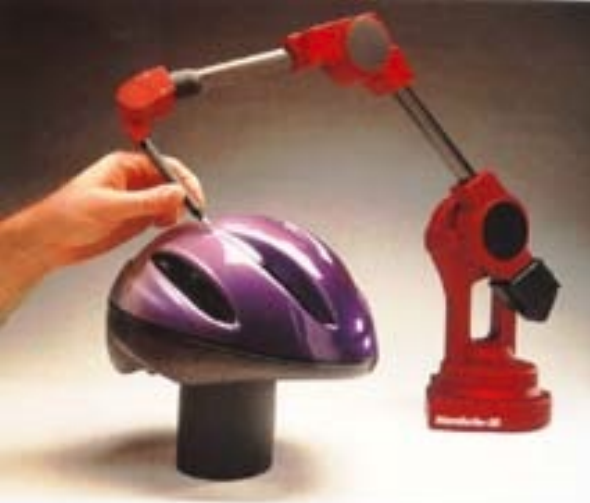
\includegraphics[width=0.8\linewidth]{images/touch_probe.png}
\end{minipage}
\begin{minipage}{0.6\textwidth}
    \centering
    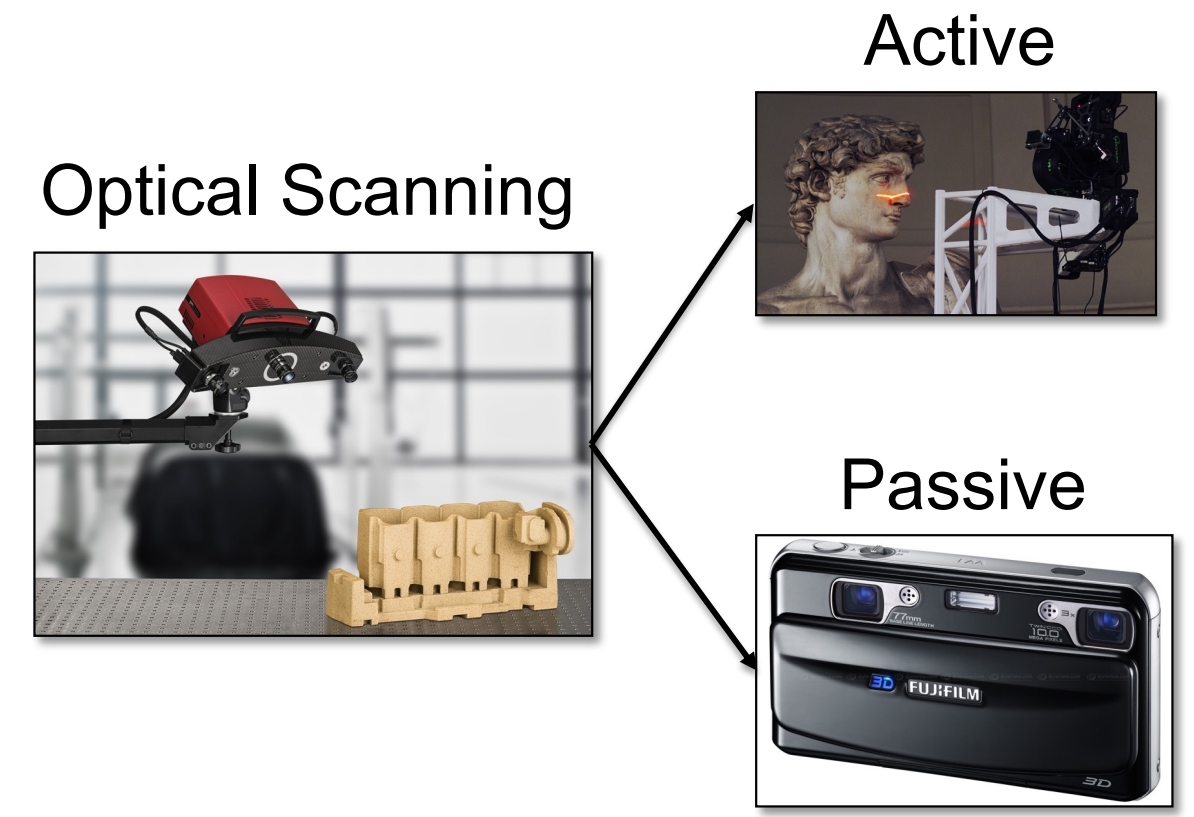
\includegraphics[width=0.9\linewidth]{images/optical_scanning.png}
\end{minipage}

\vspace{10px}

There's two main types of Optical Scanning, those are \textbf{Active} and \textbf{Passive} scanning.

\newpage

\begin{defin}[Active Scanning]{thm:active-scanning}
    \textbf{Active Scanning} is where the scanner has a light source that is controllable such as a laser
    or IR.
\end{defin}


\textbf{Examples of Active systems}

\vspace{10px}

\begin{addmargin}[20px]{20px}
    \textbf{LIDAR} - Measures the time it takes for a laser beam to hit the object and come back to the sensor.

    \vspace{5px}

    \textbf{Triangulation Laser} - Projected laser beam is photographed, giving the distance of the pattern.
    For example a line may be projected horizontally onto the subject and the deformation of the line gives 
    the distance. (Shown in the active optical scanning image above)
\end{addmargin}

\begin{defin}[Passive Scanning]{thm:passive-scanning}
    \textbf{Passive Scanning} is where the system only has a scanner and there is no control over the
    environment and the object poses.
\end{defin}

\begin{figure}[!ht]
    \centering
    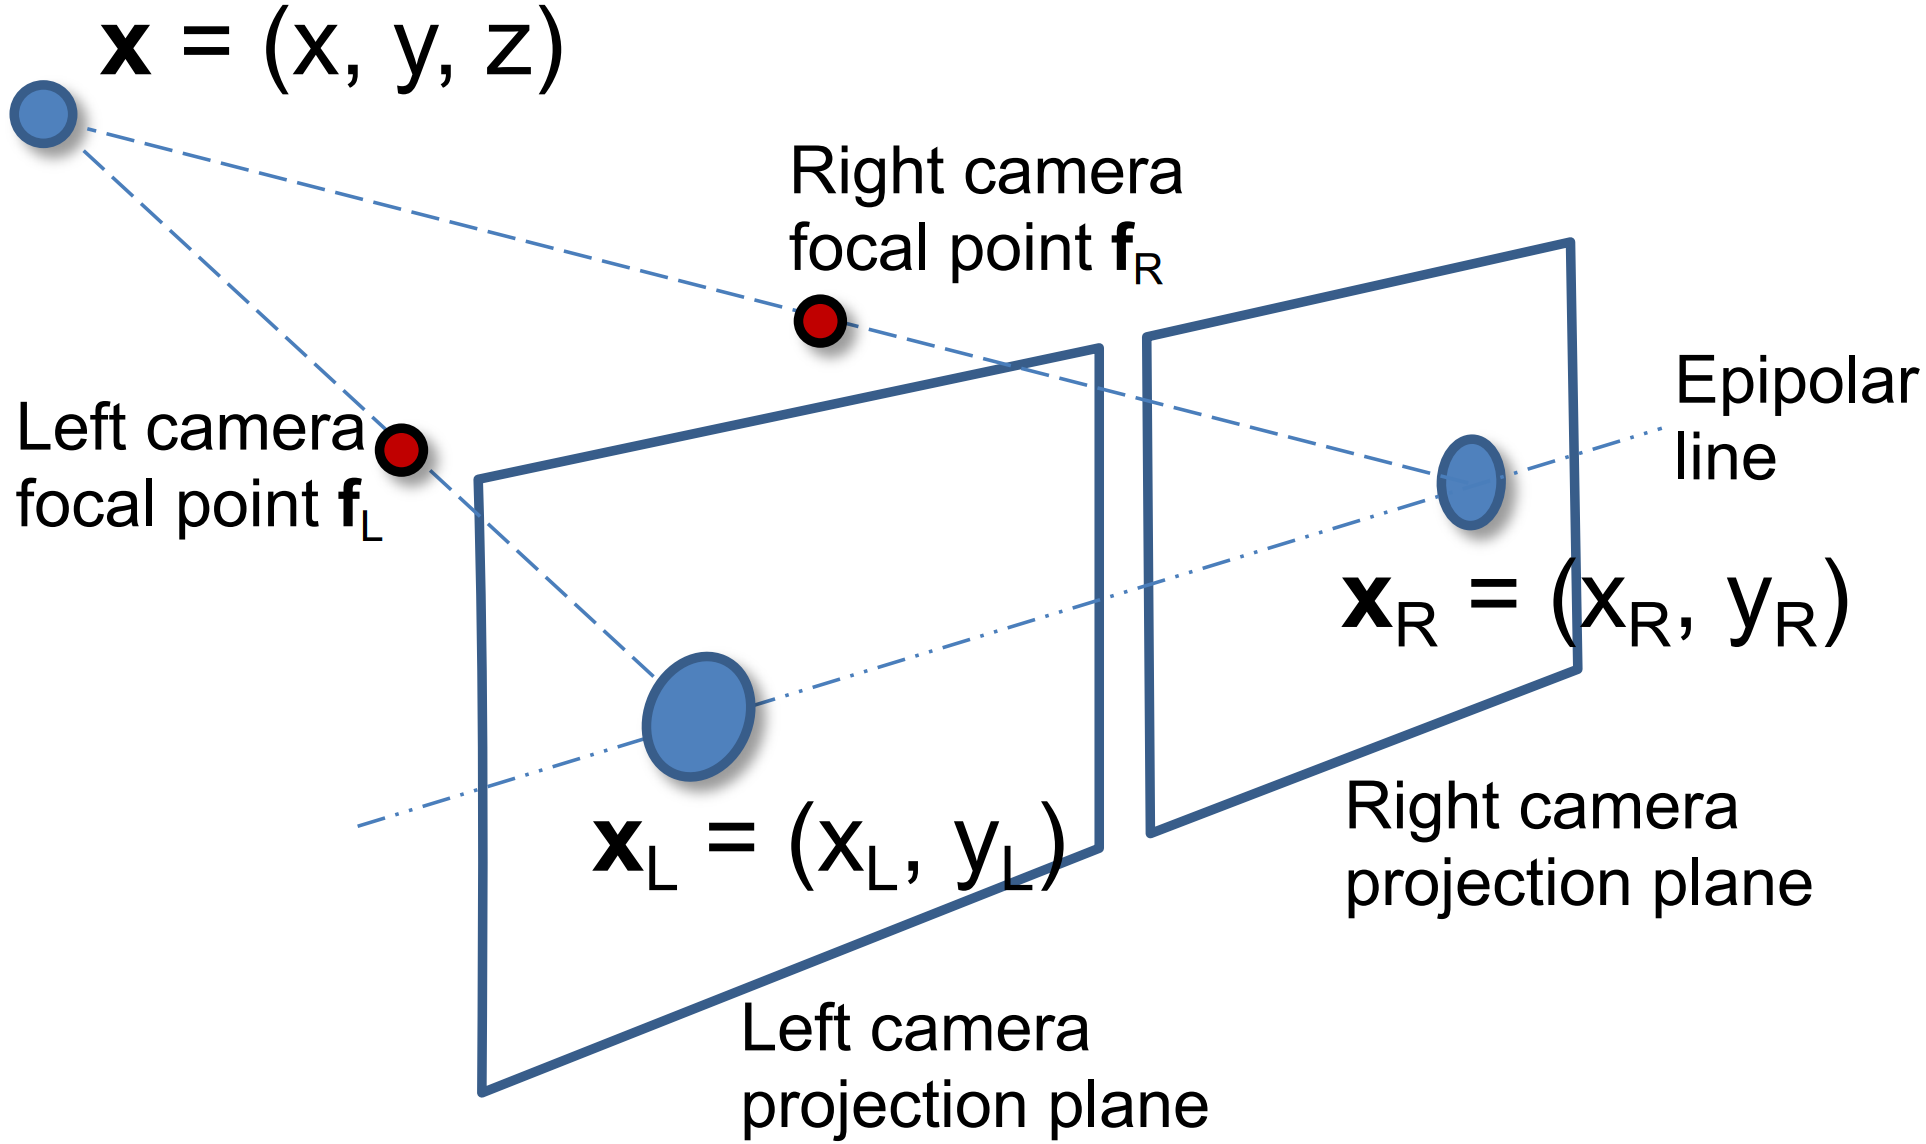
\includegraphics[width=0.5\linewidth]{images/passive_scanning.png}
\end{figure}

\vspace{10px}

The idea is you have multiple cameras typically RGB colour cameras, at least two. And then the rotation of each
camera with respect to each other. Each point \(\text{\textbf{x}}\) maps to two different points, \(\text{\textbf{x}}_{\text{L}}\)
and \(\text{\textbf{x}}_{\text{R}}\). We can then find \(\text{\textbf{x}}\) by intersecting the lines connecting
\(\mathbf{f}_{\text{L}}\) and \(\text{\textbf{x}}_{\text{L}}\), and \(\mathbf{f}_{\text{R}}\) and \(\text{\textbf{x}}_{\text{R}}\).

\vspace{5px}

This assumes we already know \(\text{\textbf{x}}_{\text{L}}\) and \(\text{\textbf{x}}_{\text{R}}\) corresponds to the same
point in 3D.

\newpage

\subsubsection{Registration}

\begin{defin}[Registration]{thm:registration}
    \textbf{Registration} is when multiple scans of a single object which yield individual point clouds 
    are brought into a common coordinate frame to create a single point cloud. There are a
    few methods such as \textbf{Iterative Closest Point Algorithms} or \textbf{Feature-Based Methods}.

    \vspace{5px}

    This is because the individual point clouds are in different coordinate frames for example
    rotated and translated.
\end{defin}

\vspace{5px}

\textbf{Iterative Closest Point Algorithms - (ICP) Algorithms}

\vspace{5px}

ICP algorithms are typically used for precise registration. The steps are below:


\begin{enumerate}
    \item Establish point-to-point correspondences
    \item Compute and apply the optimum rotation and translation
    \item Iterate the previous steps
\end{enumerate}

\begin{figure}[!ht]
    \centering
    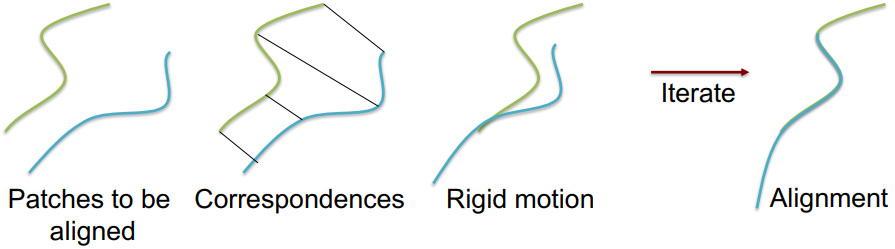
\includegraphics[width=0.8\linewidth]{images/ICPA.png}
\end{figure}

\textbf{Feature-Based Methods}

\vspace{5px}

If the rotation and or translation of the patches are initially really off, then establishing the 
correspondences for ICP algorithms is not easy and most likely will fail to align the patches.

Feature-Based Methods compute rotation and translation invariant descriptors for points and match those.

\begin{figure}[!ht]
    \centering
    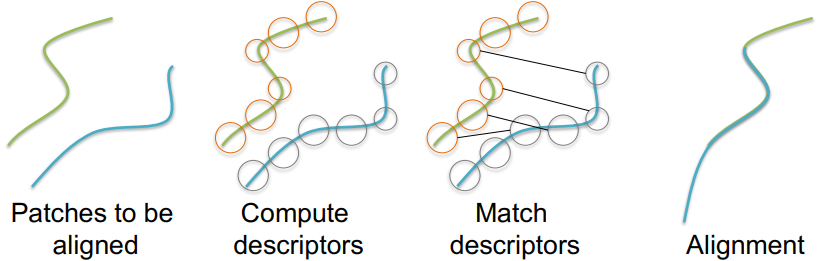
\includegraphics[width=0.8\linewidth]{images/feature_based.png}
\end{figure}

Normally we use curvature of the surface or the curve in this example for these features.

\newpage

\subsubsection{Pre-Processing}

\vspace{5px}

\begin{defin}[Pre-Processing]{thm:pre-processing}
    \textbf{Pre-Processing} is the act of cleaning, repairing, resampling of the point clouds.
\end{defin}


\vspace{5px}

Accurate and efficient reconstructions of surfaces fundamentally depends on how we distribute points on
the surface to represent the surface.

\vspace{5px}

There are extensions of the sampling theorem to irregular sampling on surfaces.

\begin{figure}[!ht]
    \centering
    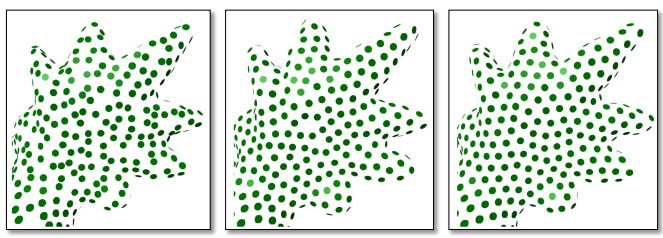
\includegraphics[width=0.5\linewidth]{images/sampling_points.png}
\end{figure}


\subsubsection{Reconstruction}

\begin{defin}[Reconstruction]{thm:reconstruction}
    \textbf{Reconstruction} is turning the point cloud to a mathematical representation of the shape.
\end{defin}

\vspace{5px}

There are two ways to reconstruct a mathematical definition of a surface.

\begin{enumerate}
    \item Connecting the sample points with lines/polygons
    \item Approximate the underlying surface for example with a least squares solution
\end{enumerate}

\begin{figure}[!ht]
    \centering
    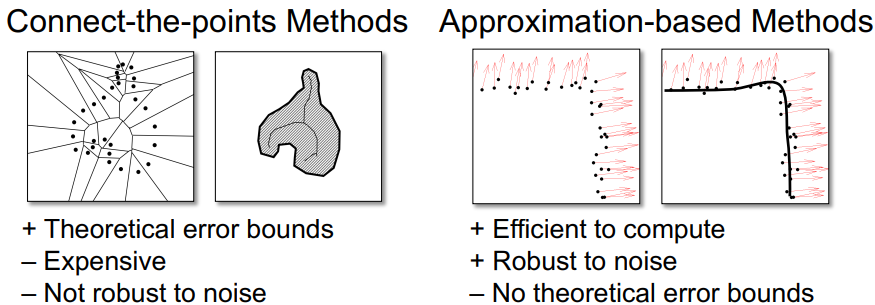
\includegraphics[width=0.5\linewidth]{images/reconstruction_two_methods.png}
\end{figure}

The connect the points creates a curve that passes through every point whereas the approximation method does not
necessarily create a curve that passes through the points.


\vspace{10px}

\textbf{Implicit Approximation}

Some of the most versatile reconstruction methods work with \hyperref[implicit-curves/surfaces]{implicit representations}


\begin{minipage}{0.3\textwidth}
    \centering
    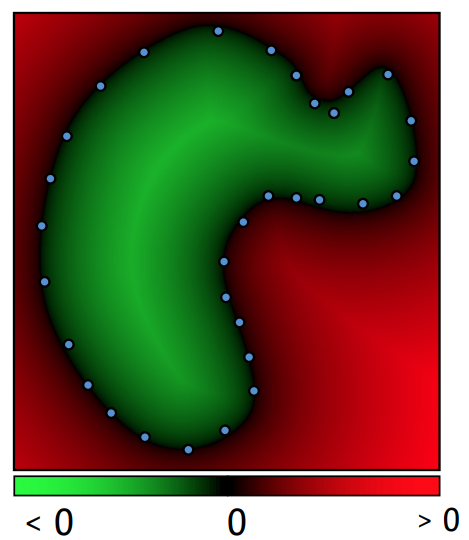
\includegraphics[width=0.9\linewidth]{images/implicit_approximation.png}
\end{minipage}
\begin{minipage}{0.6\textwidth}
    We try to estimate the points as an implicit function then extract the zero set 
    \[
        \{ \text{\textbf{x}} | f(\text{\textbf{x}}) = 0 \}
    \]
\end{minipage}




\vspace{5px}

\newpage

\subsection{Texture Mapping}

Once the surface has been reconstructed we can add colour and specific details using texture mapping.

To do this it requires parametrizing the surface, i.e. finding a mapping from a plane to the surface.

\vspace{5px}

The (\(u,v\)) coordinates live on the image plane. For each (\(u,v\)), we have the corresponding point 
(\(x, y, z\)). We can assume the texture space is a unit square and define a map \(P\) from the surface
to this square.

\begin{gather*}
    P\, : M \to [0,1] \times [0,1] \\
    P(x,y,z) = (u,v)
\end{gather*}

\vspace{5px}

Then there is a further mapping from the (\(u,v\)) space to an attribute, e.g. colour.

This mapping will be denoted by \(T\).

\begin{gather*}
    T \, : [0,1] \times [0,1] \to  \text{RGB} \\
    T(u,v) = (\text{r},\text{g},\text{b})
\end{gather*}

\vspace{5px}

These two individual mappings can be combined to create a final mapping which provides us with a colour
for each point on the surface.

\[
    \text{Colour}(x,y,z) = T(P(x, y, z))
\]

\subsubsection{Parametrization}

The main part here is the parameterization \(P\). In general, it is impossible to have a distortion-free
map from a plane to a surface in 3D. Therefore we need to decide on what distortion we allow for.

\begin{figure}[!ht]
    \centering
    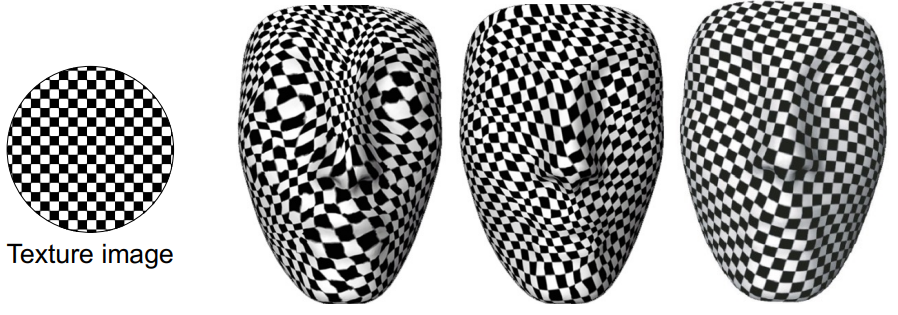
\includegraphics[width=0.5\linewidth]{images/distortion_example.png}
\end{figure}


To define the properties of distortion, we first write \(\mathbf{p}\) as three functions, one for each
component as we did before. Such a parameterization implies a map from \(uv\)-space to those in 3D space.

\[
    \mathbf{p}(u,v) = 
    \begin{pmatrix}
        x(u,v) \\ 
        y(u,v) \\
        z(u,v)
    \end{pmatrix}\!, \ (u,v) \in \mathbb{R}^2
\]

\def\E{\mathbf{p}_{u}^T \mathbf{p}_{u}}
\def\F{\mathbf{p}_{u}^T \mathbf{p}_{v}}
\def\G{\mathbf{p}_{v}^T \mathbf{p}_{v}}


We can then define the so-called \textbf{First Fundamental} form which is the 2\(\times\)2 matrix 
consisting of dot products of derivatives with respect to \(u\) and \(v\). 

\begin{minipage}{0.435\textwidth}
    \[
        \mathbf{p}_u = \frac{\partial \mathbf{p}(u,v)}{\partial u}, \ \mathbf{p}_v = \frac{\partial \mathbf{p}(u,v)}{\partial v}
    \]
    \[
        \mathbf{I} = 
        \begin{bmatrix}
            E & F \\
            F & G
        \end{bmatrix}
        = 
        \begin{bmatrix}
            \E & \F \\[6pt]
            \F & \G
        \end{bmatrix}
    \]
\end{minipage}
\begin{minipage}{0.435\textwidth}
    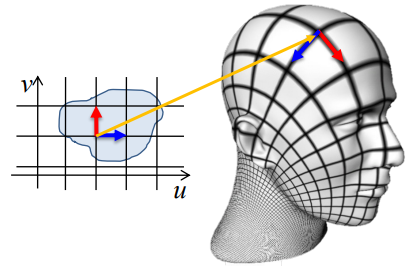
\includegraphics[width=1\linewidth]{images/parameterization_distortion.png}
\end{minipage}

( \(^T\) denotes the dot product, implying the transpose operator followed by matrix multiplication)

\vspace{10px}

This matrix measures the angle and length change in different terms.

The area distortion can also be expressed in terms of these terms. It is defined as the change in areas when
applying the map.

\begin{align*}
    \text{Angle Change} &= F = \F \\
    \text{Length Change} &= G = \G
\end{align*}

and 

\begin{defin}[Area Distortion]{thm:area-distortion}
    \[
        \text{\textbf{Area Distortion:}} \ {dA} = \sqrt{EG - F^2} {du}\,{dv}
    \]
\end{defin}


\begin{defin}[Conformal Parametrization]{thm:conformal-parameterization}
    \textbf{Conformal} maps preserve angles such that for example squares map to squares with right angles
    on the surface. For conformal maps, the \textbf{First Fundamental} form is the identity matrix.

    \vspace{5px}

    In practice we can typically compute approximately conformal maps for parameterization.
\end{defin}

\[
    \mathbf{I} = 
    \begin{bmatrix}
        \E & \F \\[6pt]
        \F & \G
    \end{bmatrix}
    = 
    \begin{bmatrix}
        \lambda & 0 \\
        0 & \lambda
    \end{bmatrix}
\]

\newpage

\subsection{Editing Geometry}

\vspace{10px}

\subsubsection{Modelling Tools}

There are many established tools to further edit geometry they depend on how you want to edit it and
for what reason.

\vspace{5px}

\begin{enumerate}
    \item Some are artistic for example via \textbf{Sculpting} where it mimics how you would do it in real life
    \item Others are for engineering related environments for example designing machine parts. \textbf{CAD/CAM}
    \item \textbf{Procedural} is where rules are defined for the geometry to be created. It is particularly
    useful in games for creating terrain or cities.
\end{enumerate}

\begin{figure}[!ht]
    \centering
    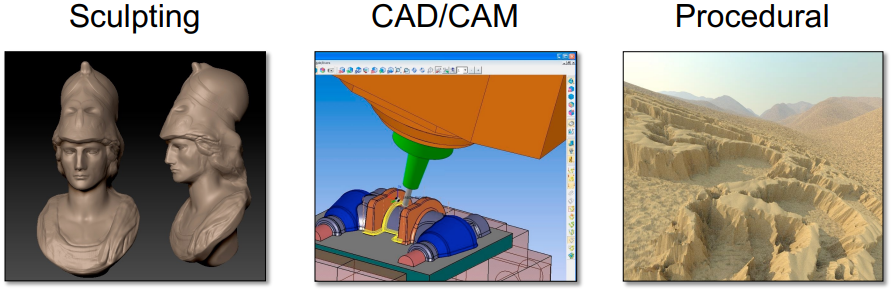
\includegraphics[width=0.8\linewidth]{images/modelling_tools.png}
\end{figure}


\subsubsection{Deformations}

\vspace{5px}

Deforming an initial surface is a typical workflow in digital modelling tools.

Such deformations can be based on low-level related characteristics for example elastic or plastic deformations
or high level deformations such as skeletal deformations.

\begin{figure}[!ht]
    \centering
    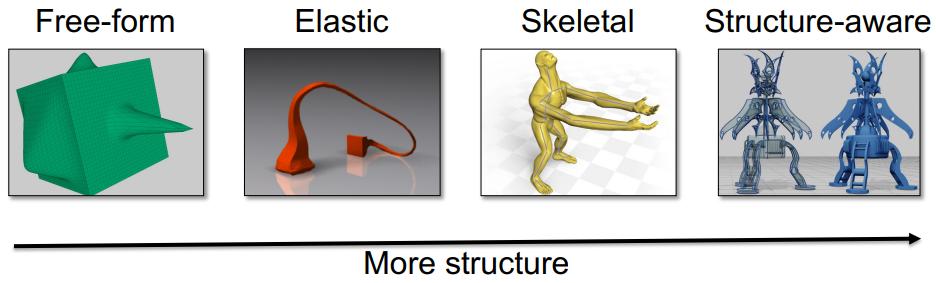
\includegraphics[width=0.8\linewidth]{images/deformations.png}
\end{figure}

\subsubsection{Cutting and Fracturing}

\vspace{5px}

\textbf{Cutting and Fracturing} through physics simulations for example
leads to changing mesh connectivity. 

This is rather difficult and one of
the reasons why connectivity-free geometry representations are useful.

\vspace{10px}

\newpage

\subsubsection{Smoothing and Filtering}

\vspace{5px}

Many algorithms exist for smoothing geometry or amplifying certain features of surfaces.

A lot of them are curvature-based, for example reducing local curvature across the mesh leads to smoothing.

\begin{figure}[!ht]
    \centering
    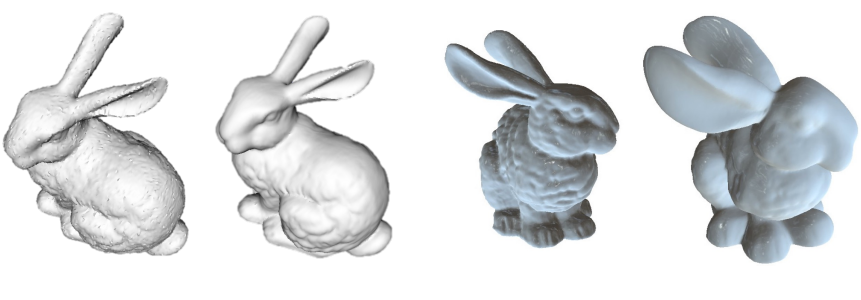
\includegraphics[width=0.5\linewidth]{images/smoothing_and_filtering.png}
\end{figure}

\vspace{10px}

\subsubsection{Compression and Simplification}

\vspace{5px}

Compression of geometric representations can be reducing the number of vertices in a mesh or quantizing the 
vertex locations, it is important for modern large data processing with billions of triangles.

\vspace{5px}

Many compression methods, like Smoothing and Filtering, also can be reduced to preserving local properties given
by curvature.


\newpage

\section{Animation}


\begin{defin}[Animation]{thm:animation}
    \textit{Technically}: \textbf{Animation} is the process of creating sequences of images

    \vspace{5px}

    \textit{Artistically}: \textbf{Animation} is the process of bringing images to life.
\end{defin}

\begin{minipage}{0.49\textwidth}
    \textbf{Things we animate:}
    \begin{enumerate}[font=\bfseries]
        \itemsep-0.1em
        \item Characters
        \item Faces
        \item Hair
        \item Elastic Materials
        \item Natural Phenomena
        \item Cloths
        \item Herds
        \item Crowds
        \item etc.
    \end{enumerate}  
\end{minipage}
\begin{minipage}{0.49\textwidth}
    \textbf{How we Animate}
    \begin{enumerate}[font=\bfseries]
        \itemsep-0.1em
        \item Key-Framing
        \item Skeletal
        \item Subspace/Parameters
        \item Physically Based
        \item Motion Capture
        \item Video Based
        \item Example Based
        \item Procedural
        \item etc.
    \end{enumerate}
\end{minipage}

\vspace{15px}

Key-framing controls given by abstract skeletons or other parameters is how animations are created.

This provides control over deformations and timing, which are both critical for creating animations.

The final complex animations are obtained by blending simpler transformations together.

\vspace{5px}

There are many ways to augment this process, but the fundamental ideas of controls and blending
transformations do not change too much.


\subsection{Considerations}

Animating requires absolute \textbf{control}.

\textbf{Efficiency} and \textbf{Style} are also tightly coupled with control.

Controlling animations with computers typically means dragging points and curves around to define deformations.


\subsection{Character Animation}

Character animation will be used a working example.

\vspace{5px}

It is the most important and generalizable way to animate objects and heavily used in industry.
It requires blending transformations, for which we need to understand some fundamental maths.

\vspace{10px}

\textbf{Animation Pipeline}

\vspace{-5px}

\begin{minipage}[t]{0.49\textwidth}
    \addtopstrut
    \begin{enumerate}[font=\bfseries, itemsep=-4px]
        \item Story boarding \vspace{-6px} 
            \begin{itemize}
                \itemsep-3px
                \item A board for setting up the story
                \item Helps planning animations
            \end{itemize}
        \item Concept Design \vspace{-6px} 
            \begin{itemize}
                \itemsep-3px
                \item Sketches for characters and environment
                \item Main features of the characters
            \end{itemize}
        \item 3D Modelling \vspace{-6px} 
            \begin{itemize}
                \itemsep-3px
                \item Moving to computers
                \item Geometry and Textures
            \end{itemize}
        \item Rigging \vspace{-6px} 
            \begin{itemize}
                \itemsep-3px
                \item Embedding animation controllers
                \item Construct a skeleton and attach additional controls
                \item Key-frame the controllers for animation
            \end{itemize}
    \end{enumerate}
    \addbottomstrut
\end{minipage}
\begin{minipage}[t]{0.435\textwidth}
    \addtopstrut
    \begin{enumerate}[font=\bfseries, itemsep=-4px]
        \setcounter{enumi}{4}
        \item Blend Shapes Creation \vspace{-6px} 
            \begin{itemize}
                \itemsep-3px
                \item Create facial expressions
                \item Used to generate other expressions via blending
            \end{itemize}
        \item Animation \vspace{-6px} 
            \begin{itemize}
                \itemsep-3px
                \item Set key-frames  for controllers
                \item Steer interpolation and timing with time controls
            \end{itemize}
        \item Post-Effects \vspace{-6px} 
            \begin{itemize}
                \itemsep-3px
                \item Other animations  (fluids, cloth, etc)
                \item Lighting and shading
                \item Rendering
            \end{itemize}
    \end{enumerate}
    \addbottomstrut
\end{minipage}

\newpage

\subsection{Rigging}

\begin{defin}[Rigging]{thm:rigging}
    A 3D model is typically represented as a surface mesh. \textbf{Rigging} is the process of attaching an 
    abstract skeleton consisting of bones and joints to the model.

    \vspace{5px}

    As the user changes the configuration of the skeleton the model is deformed accordingly
\end{defin}

\textbf{Rigging} in short is the process of attaching a skeleton to a model.

\vspace{10px}

The first step to rigging is positioning the skeleton so that semantically corresponding parts of the skeleton
and the model are close, i.e. the forearm bone and the forearm are roughly aligned.

\vspace{5px}

The next step is defining a function on the surface model for each bone, which is colour coded below

\begin{figure}[!ht]
    \centering
    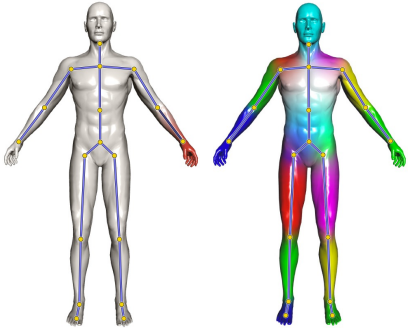
\includegraphics[width=0.5\linewidth]{images/skeleton_coloured.png}
\end{figure}


If we look closer at the skeleton we have bones, joints, and the hierarchy of these in a skeleton.
(This is just an abstract look at a skeleton for the purpose of user interpretation of motion for motion
control)

\vspace{5px}

The hierarchy is important for controlling the skeleton, e.g. if you pick the hip joint and change the 
location of it, the legs are moving along with it.

\begin{figure}[!ht]
    \centering
    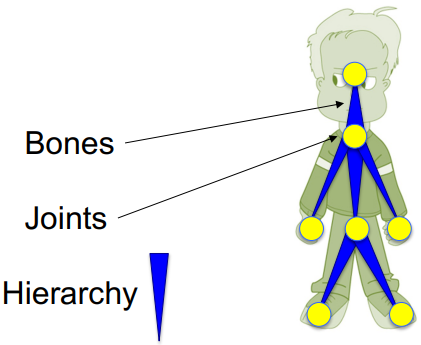
\includegraphics[width=0.3\linewidth]{images/skeleton_hierarchy.png}
\end{figure}

A rotation and a translation is stored on each bone or joint. We can assume they are stored on bones. As the
user transforms bones via the mouse or another control these transformations are updated.

\vspace{5px}

We can store the rotations as matrices \(\mathbf{R}_{i}\) and vectors \(t_i\) as translations.

\vspace{5px}

Note: This means each bone is rigid so no bending.

\vspace{10px}

The second step of rigging is attaching each bone to the 3D model. This means computing a weighting function
for each bone that determines how much the transformation on a bone is affecting a given point on
the surface of the model

\newpage

To see how this works we're going to look at a simple case: A simple mesh with two bones and 3 joints.

\begin{figure}[!ht]
    \centering
    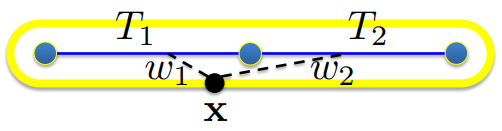
\includegraphics[width=0.5\linewidth]{images/skeleton_simple_model.png}
\end{figure}

As we change the transformation \(\mathbf{T}_i\), (The rotation and translation), the mesh should deform
accordingly.

\vspace{5px}

To compute a new position of a given point \(\text{\textbf{x}}\) on the mesh.

\begin{enumerate}
    \item Blend the transformations with the weights stored \(w_i\). (Denoted by the avg function below)
    \item Apply the transformation to the point \(\text{\textbf{x}}\) to get the new corresponding point
    on the deformed model.
\end{enumerate}


\[
    T(\text{\textbf{x}}) = \operatorname{avg}(T_1, T_2, w_1, w_2)
\]

\subsubsection{Linear Blend Skinning}

One way to represent the transformations is via 4\(\times\)4 transformation matrices \(\mathbf{T}_i\),
and blending via a linear combination of those.

\vspace{5px}

Each matrix stores both the rotation and translation.

\vspace{5px}

The final blended transformation is then applied to the point \(\text{\textbf{x}}\) in homogenous
coordinates, i.e. \(\text{\textbf{x}} = [x, y, z, 1]^T\)

\begin{gather*}
    \mathbf{T}(\text{\textbf{x}}) = w_1(\text{\textbf{x}}) \mathbf{T}_1 + w_2(\text{\textbf{x}}) \mathbf{T}_2\\
    \text{\textbf{x}}' = \mathbf{T}(\text{\textbf{x}})\text{\textbf{x}}
\end{gather*}

\[
    \mathbf{T} = \begin{bmatrix}
        \mathbf{R}_{1,1} & \dots & \mathbf{R}_{1,3} & t_1 \\
        \vdots & \ddots & \vdots & \vdots \\
        \mathbf{R}_{3,1} & \dots & \mathbf{R}_{3,3} & t_3 \\
        0 & 0 & 0 & 1
    \end{bmatrix} =
    \begin{bmatrix}
        \mathbf{R} & & & \!\!\mathbf{t}\\
        0 & \!\!\!0 & \!\!\!0 & \!\!\!1
    \end{bmatrix}
\]

\vspace{5px}

The main problem with linear blend skinning is that it assumes no structure for rotation matrices.

(In general, linear combinations of rotation matrices are not valid rotation matrices)

\[
    w_1 \mathbf{T}_1 + w_2 \mathbf{T}_2
\]

\begin{itemize}[itemsep=-4px]
    \item \(w_1 \mathbf{t}_1 \: \, + w_2 \mathbf{t}_2 \; \, \) is a valid translation
    \item \(w_1 \mathbf{R}_1 + w_2 \mathbf{R}_2\) is \textbf{not} a valid rotation matrix
\end{itemize}

For a rotation matrix to be valid it should satisfy the following two properties

\begin{enumerate}[itemsep=0px]
    \item {\makebox[0.5\textwidth][l]{Its transpose is equal to its inverse} \(\mathbf{R}^T=\mathbf{R}^{-1}\)}
    \item {\makebox[0.5\textwidth][l]{Its determinant is equal to 1} \(\det \mathbf{R}= 1\)}
\end{enumerate}

For linear blending though this is not the case.

\begin{alignat*}{3}
    &(w_1 \mathbf{R}_1 &&+ w_2 \mathbf{R}_2&&)^T \\
    = &(w_1 \mathbf{R}_1^T &&+ w_2 \mathbf{R}_2^T&&) \\
    \neq &(w_1 \mathbf{R}_1 &&+ w_2 \mathbf{R}_2&&)^{-1}
\end{alignat*}

\newpage

In practice, invalid matrices lead to volume loss, especially around the joints where the blending is
strongest.

\begin{figure}[!ht]
    \centering
    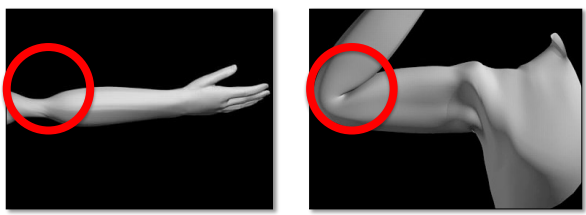
\includegraphics[width=0.5\linewidth]{images/linear_blend_skinning_problems.png}
    \caption*{Left: \textbf{Candy-Wrapper} artefact \hspace{20px} Right: \textbf{Elbow Collapse} artefact}
\end{figure}

We can visualize what is going wrong by considering the subspace 
(it is a manifold) of rotation matrices in the 9 dimensional space of all 3x3 matrices.
A linear combination of rotation matrices will not necessarily lie on this manifold.
Instead, what we want is the shortest path that respects the manifold of rotation matrices.

\begin{figure}[!ht]
    \centering
    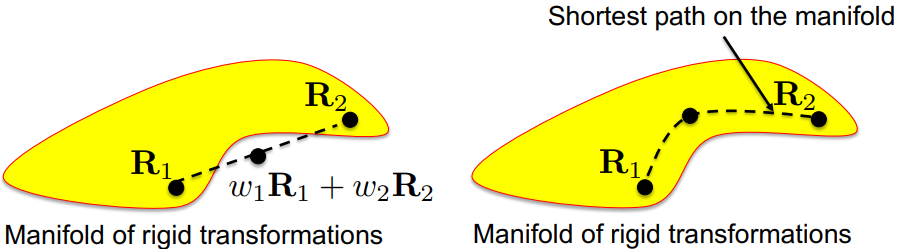
\includegraphics[width=0.5\linewidth]{images/manifold_of_rigid_transformations.png}
\end{figure}

This manifold is called SO(3) and is given by the two condition on valid rotation matrices we have seen.

\vspace{10px}

\textbf{Manifold of Rotations - SO(3)}

\begin{gather*}
    \mathbf{R}^T=\mathbf{R}^{-1}\\
    \det \mathbf{R}= 1
\end{gather*}


\textbf{Manifold of Rigid Transformations - SE(3)}

\begin{center}
    \begin{minipage}{0.2\textwidth}
        \begin{gather*}
            \mathbf{R}^T=\mathbf{R}^{-1}\\
            \det \mathbf{R}= 1
        \end{gather*}
    \end{minipage}
    \begin{minipage}{0.2\textwidth}
        \[
            \mathbf{T} = 
            \begin{bmatrix}
                \mathbf{R} & & & \!\!\mathbf{t}\\
                0 & \!\!\!0 & \!\!\!0 & \!\!\!1
            \end{bmatrix}
        \]
    \end{minipage}  
\end{center}

In summary, it is hard to generate valid rigid transformations with linear combinations if we work with the matrix
representation of transformations.
Instead, we will utilize an alternative representation: \textbf{dual quaternions}.

\newpage

\subsection{Quaternions}

\begin{defin}[Quaternion]{thm:quaternion}
    \[
        \mathbf{q} = \cos \left(\frac{\theta}{2}\right) + \mathbf{s} \sin\left(\frac{\theta}{2}\right)
    \]

    \vspace{-20px}

    \begin{center}
        \begin{alignat*}{2}
            \mathbf{q}& \quad &&\text{is the quaternion}\\
            \theta& &&\text{is the \textbf{rotation angle}}\\
            \mathbf{s}& &&\text{is the \textbf{rotation axis}}
        \end{alignat*}
    \end{center}
\end{defin}


The rotation axis \(\mathbf{s}\) is represented with an extension of imaginary numbers, denoted with 
\(i,j,k\). The rotation axis is a unit vector.
\vspace{-5px}
\begin{gather*}
    \mathbf{s} = s_i i + s_j j + s_k k \\
    s^2_i + s^2_j + s^2_k = 1 \\
    i^2 = j^2 = k^2 = ijk = -1
\end{gather*}

\subsubsection{Operations on Rotation Quaternions}

\begin{center}
    (For quaternions that have a norm of 1)
\end{center}

\textbf{Conjugate}

\vspace{5px}

The conjugate has the same meaning as for imaginary number i.e. the non-real part (in this case is \(\mathbf{s}\))
is negated.

\[
    \mathbf{q}^* = \cos \left(\frac{\theta}{2}\right) - \mathbf{s} \sin\left(\frac{\theta}{2}\right) =
    \cos \left(- \frac{\theta}{2}\right) + \mathbf{s} \sin\left(- \frac{\theta}{2}\right)
\]

\textbf{Inverse}

\vspace{5px}

\[
    \mathbf{q}^{-1} = \mathbf{q}^*
\]

\textbf{Multiplication}

\vspace{5px}

Composing rotations is done by multiplying quaternions. Multiplication is carried out by using the following rules
\vspace{-5px}
\begin{alignat*}{5}
    &ij &&= k \qquad &&ji &&= -k\\
    &jk &&= i \qquad &&kj &&= -i\\
    &ki &&= j \qquad &&ik &&= -j
\end{alignat*}
\[
    i^2 = j^2 = k^2 = -1
\]

\[
    \mathbf{q}_1 \mathbf{q}_2 = (a_1 + b_1 i + c_1 j + d_1 k)(a_2 + b_2 i + c_2 j + d_2 k)
\]

Multiplying a quaternion with its conjugate gives us the norm, which is 1 for the case of
quaternions representing rotations.

\vspace{5px}

\textbf{Norm}

\[
    \lVert q \rVert^2 = \mathbf{q}\mathbf{q}^* = \cos^2 \left(\frac{\theta}{2}\right) + 
    \lVert \mathbf{s} \rVert^2 \sin\left(\frac{\theta}{2}\right) = 1
\]


% \textbf{Derivation}:

% \vspace{5px}

% \begin{align*}
%     \mathbf{q}\mathbf{q}^* &= \left(\cos \left(\frac{\theta}{2}\right) + \mathbf{s} \sin\left(\frac{\theta}{2}\right)\right)
%     \left(\cos \left(\frac{\theta}{2}\right) - \mathbf{s} \sin\left(\frac{\theta}{2}\right)\right)\\
%     &= \cos^2 \left(\frac{\theta}{2}\right) +  \mathbf{s} \sin\left(\frac{\theta}{2}\right)
% \end{align*}


\textbf{Power}

\vspace{5px}

\[
    \mathbf{q}^t = e^{t \log \mathbf{q}}
\]
\[
    \log \mathbf{q} = \frac{\theta}{2} \mathbf{s} \qquad e^\mathbf{q} = \cos \lVert \mathbf{q} \rVert
    + \frac{\mathbf{q}}{\lVert \mathbf{q} \rVert }  \sin \lVert \mathbf{q} \rVert 
\]
\begin{center}
    (\(e^{\mathbf{q}}\) only holds when the scalar part of the quaternion is 0)
\end{center}

\textbf{Applying to Location Vectors}

\vspace{5px}

To apply a quaternion to a vector to rotate it, we first need to write the vector in \(i,j,k\) space.

The \(\mathbf{v}'\) is then the rotated version of \(\mathbf{v}\)

\begin{alignat*}{2}
    &\mathbf{v} &&= v_i i + v_j j + v_k k \\
    &\mathbf{v}' &&= \mathbf{qvq}^* 
\end{alignat*}

\textbf{Blending Quaternions}

\vspace{5px}

For the special case that the axes of rotation are the same for both quaternions, their blending/interpolation
is the interpolation of the angle of rotation.

\[
    \mathbf{s} = \mathbf{s}_1 = \mathbf{s}_2
\]

\[
    \operatorname{interpolate}(\mathbf{q}_1, \mathbf{q}_2, t)
\]

\vspace{-15px}

\begin{alignat*}{3}
    \theta&(t) &&= \ &&(1-t)\theta_1 + t \theta_2 \\
    \mathbf{q}&(t) &&= &&\cos \left(\frac{\theta(t)}{2}\right) + \mathbf{s} \sin\left(\frac{\theta(t)}{2}\right)
\end{alignat*}

\textbf{Spherical Blending}:

\vspace{5px}

For the general case though we use the so-called spherical blending for two quaternions.

\vspace{5px}

For \(t=0\) we get \(\mathbf{q}_1\), and for \(t=1\) we get \(\mathbf{q}_2\) as expected.

\[
    \mathbf{s}_1 \neq \mathbf{s}_2
\]

\[
    (\mathbf{q}_2 \mathbf{q}_1^*)^t \mathbf{q}_1
\]


\textbf{Blending More Than Two Quaternions}:

There is no closed form solution. A good approximation is a weighted sum of quaternions.

(This is the reason why we care about quaternions. In contrast to matrix based representations 
quaternion linear blending does not lead to volume loss and other artefacts)

\[
    \mathbf{q}_{1}, \cdots, \mathbf{q}_{n} \qquad w_{1}, \cdots, w_{n}
\]

\[
    \mathbf{b} = \sum_{i=1}^{n}w_i \mathbf{q}_i
\]

\newpage

\subsubsection{Dual Quaternions}

\begin{defin}[Dual Numbers]{thm:dual-numbers}
    Dual numbers have a real part and a \textbf{dual} part. The dual number \(\epsilon\) has the property

    \[
        \epsilon^2 = 0 \qquad \wedge \qquad \epsilon \neq 0
    \]

    \vspace{-10px}

    \[
        \hat{x} = x_0 + \epsilon x_\epsilon
    \]

    This property leads to cancellation of higher order terms in multiplication. For an example 
    multiplication of two dual numbers.
    \begin{align*}
        (&a_0 + \epsilon a_\epsilon)(b_0 + \epsilon b_\epsilon) \\
        = \ \ &a_0b_0 + \epsilon(a_0 b_\epsilon + a_\epsilon b_0)
    \end{align*}
\end{defin}

\begin{defin}[Dual Quaternions]{thm:dual-quaternions}
    For dual quaternions the component of the axis \(\mathbf{s}\) become dual numbers.

    \vspace{5px}

    All operations and expressions we are interested in stay the same.

    \[
        \hat{q} = \cos \left(\frac{\hat{\theta}}{2}\right) + \mathbf{\hat{s}} \sin\left(\frac{\hat{\theta}}{2}\right)
    \]

    In particular, we still have the linear combination as a good approximation of proper shortest path
    blending.

    \[
        \mathbf{\hat{b}} = \sum_{i=1}^{n} w_i \mathbf{\hat{q}}_i
    \]
\end{defin}

These dual quaternions now mean we can represent a rotation and a translation with a rotation around the axis
\(\mathbf{s}\) and a translation along the same axis.

\begin{figure}[!ht]
    \centering
    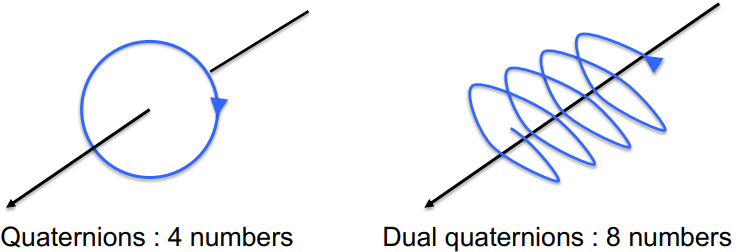
\includegraphics[width=0.4\linewidth]{images/dual_quaternions_vs_quaternions.png}
\end{figure}

There is one thing that was brushed over: only normalized quaternions/ dual quaternions represent
valid rotations/ rigid transformations.

\vspace{5px}

With normalization, we always get dual quaternions representing valid rigid transformations.

\[
    \mathbf{\hat{b}} = \sum_{i=1}^{n} w_i \mathbf{\hat{q}}_i
\]

Only generates valid transformations iff its normalized.

\[
    \mathbf{\hat{b}} = \frac{\sum_{i=1}^{n} w_i \mathbf{\hat{q}}_i}
    {\lVert \sum_{i=1}^{n} w_i \mathbf{\hat{q}}_i \rVert}
\]


An important property of the approximate blending is that it is invariant to coordinate change:
If we first transform all dual quaternions with the same transformations and then blend the representing
quaternions we get the same result as first blending them and then applying the transformation.

\vspace{5px}

This follows from the property: \(\Sigma w_i \mathbf{\hat{q}} \mathbf{\hat{q}}_i = \mathbf{\hat{q}} \Sigma \mathbf{\hat{q}}_i\)

\vspace{10px}

This simple linear blending stays very close to the shortest path blending on SE(3), the manifold of 
valid rigid transformations.

\newpage

\subsubsection{Challenges of Transformations}

Apart from the transformation representation, there are challenges with how we compute the weight for 
blending. There are several intuitive properties.

Blending Transformations - We use Dual Quaternions

\vspace{5px}

Weights \(w_i(\text{\textbf{x}})\)

\begin{itemize}
    \item Shape Adaptive
    \item Intuitive Deformations
    \item Smooth Deformations
\end{itemize}

The first property is partition of unity. This is important for volume preservation.

\[
    \sum_{i=1}^{n} w_i (\text{\textbf{x}}) = 1
\]

The second property is smoothness of weights. This ensures we get smooth deformations without artefacts.

\vspace{5px}

Finally the last property is shape-awareness which leads to local influence with respect to respect to the
deformed shape and is important for intuitive control.

\begin{figure}[!ht]
    \centering
    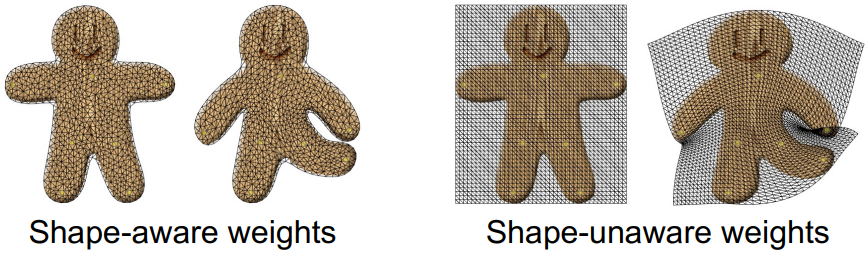
\includegraphics[width=0.5\linewidth]{images/shape_aware_vs_shape_unaware.png}
\end{figure}


\newpage

\section{The Rendering Equation}

\subsection{Basic Definitions}

\textbf{Angle}: 

\begin{minipage}{0.435\textwidth}
    \[
        \theta = \frac{l}{r}
    \]
    \begin{center}
        A circle is \(2\pi\) radians
    \end{center}
\end{minipage}
\begin{minipage}{0.435\textwidth}
    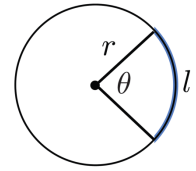
\includegraphics[width=0.3\linewidth]{images/radians.png}
\end{minipage}

\textbf{Solid Angle}:

\begin{minipage}{0.435\textwidth}
    \[
        \Omega = \frac{A}{r^2}
    \]
    \begin{center}
        A sphere is \(4\pi\) steradians
    \end{center}
\end{minipage}
\begin{minipage}{0.435\textwidth}
    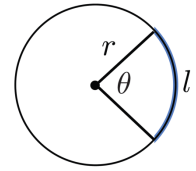
\includegraphics[width=0.3\linewidth]{images/radians.png}
\end{minipage}

\textbf{Direction}

\vspace{5px}

A point on the unit sphere parameterized by two angles \(\theta\) as zenith and \(\phi\) as azimuth.


\begin{minipage}{0.6\textwidth}
    \begin{alignat*}{3}
        &\vec{w} &&= (\theta, \phi)\\[5px]
        &\vec{w}_x &&= \sin \theta \cos \phi\\
        &\vec{w}_y &&= \sin \theta \sin \phi\\
        &\vec{w}_z &&= \cos \theta\\ 
    \end{alignat*}
\end{minipage}
\begin{minipage}{0.3\textwidth}
    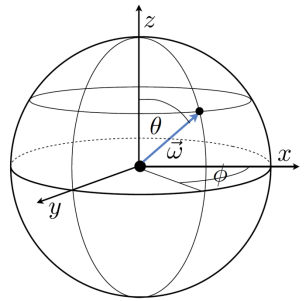
\includegraphics[width=0.8\linewidth]{images/direction.png}
\end{minipage}

\[
    \text{latitude} = \frac{90}{\pi} (\pi-\theta) \qquad \qquad \text{longitude} = \frac{90}{\pi} \phi
\]

\vspace{5px}

\textbf{Differential Solid Angle}

\vspace{5px}

Differential version of an area on a sphere is defined by considering a very small square on the sphere.
The differential solid angle can then be defined by dividing the differential area by squared radius of 
the sphere.

\vspace{5px}

(Note that we denote the differential solid angle with the same symbol as direction.)

\vspace{10px}

Integrating the differential solid angle gives the area of the unit sphere as expected.

\begin{minipage}{0.6\textwidth}
    \begin{alignat*}{2}
        &dA &&= (r d \theta) (r \sin \theta \, d \phi)\\
        &d \vec{w} &&= \frac{dA}{r^2} = \sin \theta \, d \theta d \phi
    \end{alignat*}

    \[
        \Omega = \int_S^2 d \vec{w} = \int_0^{2\pi} \int_0^{\pi} \sin \theta \, d \theta \phi = 4\pi
    \]
\end{minipage}
\begin{minipage}{0.3\textwidth}
        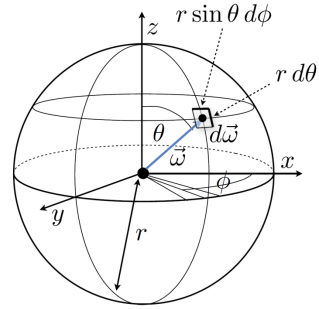
\includegraphics[width=0.9\linewidth]{images/diff_solid_angle.png}
\end{minipage}

\newpage

\subsubsection{Light}

\begin{defin}[Light]{thm:light}
    \textbf{Light} can be a mixture of many wavelengths

    \vspace{5px}

    Assume \textbf{Light} consists of photons each with:
    \begin{center}
        \begin{itemize}[label={--}, itemsep=-4px]
            \item \textbf{x} : Position
            \item \(\vec{w}\) : Direction of Motion
            \item \(\lambda\) : Wavelength
        \end{itemize}
    \end{center}

    Each Photon has an energy of: {\Large\(\frac{hc}{l}\)}

    \begin{itemize}[label={--}, itemsep=-4px]
        \item \(h \approx 6.63 \times 10^{-34} m^2 kg / s\) : Planck's constant
        \item \(c = 299,792,458m / s\) : Speed of Light in a vacuum
        \item With unit Joule \([Joule (J)] = kg m^2 / s^2\) 
    \end{itemize}
    We measure light by counting photons.
\end{defin}

\textbf{Spectral Power Distribution (SPD)}
\begin{itemize}[itemsep=-4px]
    \item \(\text{P}(\lambda) = \) intensity at wavelength \(\lambda\)
    \item Intensity as a function of wavelength
\end{itemize}

We perceive these distributions as colours.

\vspace{5px}

\subsection{Radiometry}

Radiometry is the measurement of electromagnetic radiation, including visible light.

\textbf{Flux} (Radiant Flux, Power)

The total amount of energy passing through a surface or space (\(A\)) per unit time.

\[
    \varPhi(A) \qquad \qquad \left[\frac{J}{s} = W\right]
\]

Examples can include: Number of photons hitting a wall per second. The number of photons leaving a 
lightbulb per second.

\vspace{10px}

\textbf{Radiant Intensity}

\vspace{5px}

Radiant intensity is defined with differential flux and solid angle. Intuitively, it is a very local 
measure of energy per unit time per solid angle.

\[
    I(\vec{w}) = \frac{d\varPhi}{d \vec{w}} \qquad \left[\frac{W}{sr}\right] \qquad
     \int_S^2 I(\vec{w}) d \vec{w}
\]


\newpage

\textbf{Radiance}

\begin{defin}[Radiance]{thm:radiance}
    \textbf{Radiance} is the most important quantity. It is energy per unit time per solid angle per unit 
    \textbf{perpendicular} area. Intuitively, due to the cosine term, it is independent of the angle the actual 
    area makes with the light direction.

    \vspace{5px}

    This makes sense because a large area that is tilted with respect to the light direction does not get 
    more flux.

    \vspace{5px}

    Radiance remains constant along a ray. 

    \vspace{5px}

    We will utilize it in the rendering equation.
\end{defin}

\begin{figure}[!ht]
    \centering
    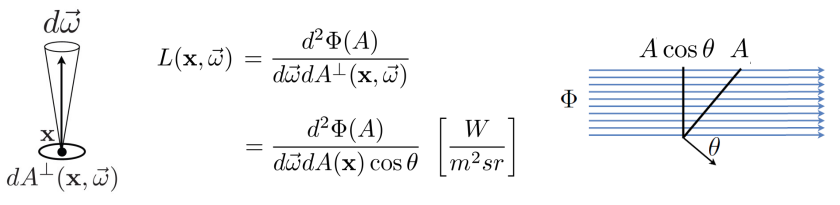
\includegraphics[width=0.8\linewidth]{images/radiant_intensity_per_perp_area.png}
\end{figure}

\newpage

\subsection{Reflection Models}

\begin{defin}[BRDF]{thm:brdf}
    % cSpell:disable
    \textbf{B}idirectional \textbf{R}eflectance \textbf{D}istribution \textbf{F}unction
    % cspell:enable

    \vspace{5px}

    \textbf{BRDF} and its variants are the most commonly used functions to represent and render light
    in a digital scene. With \textbf{BRDF}, we only consider reflection, so no light passes through any
    surface.

    \vspace{5px}

    Surfaces only reflect

    \begin{minipage}{0.5\textwidth}
        \[
            f_r(\text{\textbf{x}}, \vec{w}_i, \vec{w}_r) = \frac{d L_r(\text{\textbf{x}}, \vec{w}_r)}
            {L_i(\text{\textbf{x}}, \vec{w}_i) \cos \theta_i \, d\vec{w}_i}
        \]

        \vspace{5px}

        \begin{alignat*}{2}
            &f_r(\text{\textbf{x}}, \vec{w}_i, \vec{w}_r) \quad &&\text{- Is the \textbf{BRDF}}\\
            &d L_r(\text{\textbf{x}}, \vec{w}_r) &&\text{- Is an infinitesimal reflected radiance}\\
            &d \vec{w}_i &&\text{- Is an infinitesimal solid angle}
        \end{alignat*}
    \end{minipage}
    \begin{minipage}{0.4\textwidth}
        \raggedleft
        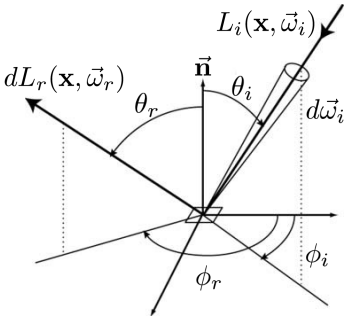
\includegraphics[width=0.8\linewidth]{images/brdf_explanation.png}
    \end{minipage}
\end{defin}

\subsubsection{Reflection and Rendering Equations}

\textbf{Reflection Equation}

\vspace{5px}

We can finally define the reflection equation, which is simply the integral form of the previous expression.
This tells us that the total reflected light for a given direction is the integral of light coming in all 
directions on the hemisphere \(H^2\) with weighting terms given by the BRDF and the cosine of the 
incoming light angle.

\vspace{5px}

(Note: that we do not integrate over the whole sphere as we assume light is only reflected off a surface.)

\def\ReflectedLight{
    \int_{H^2} f_r(\text{\textbf{x}}, \vec{w}_i, \vec{w}_r)L_i(\text{\textbf{x}}, \vec{w}_i) \cos \theta_i \, d \vec{w}_i
}

\begin{align*}
    f_r(\text{\textbf{x}}, \vec{w}_i, \vec{w}_r) &= \frac{d L_r(\text{\textbf{x}}, \vec{w}_r)}
            {L_i(\text{\textbf{x}}, \vec{w}_i) \cos \theta_i \, d\vec{w}_i}\\
    f_r(\text{\textbf{x}}, \vec{w}_i, \vec{w}_r)L_i(\text{\textbf{x}}, \vec{w}_i) \cos \theta_i \,  
        &= \frac{d L_r(\text{\textbf{x}}, \vec{w}_r)}{d\vec{w}_i}\\
    \ReflectedLight &= L_r(\text{\textbf{x}}, \vec{w}_r)
\end{align*}

\begin{defin}[Reflection Equation]{thm:reflection-equation}
    The reflected radiance due to incident illumination from all directions

    \[
        L_r(\text{\textbf{x}}, \vec{w}_r) = \ReflectedLight
    \]
\end{defin}

\textbf{Rendering Equation}

\vspace{10px}

The step to got from reflectance to rendering equation is adding a term that accounts for potentially
emitted light. This ensures that energy is conserved.

\begin{defin}[The Rendering Equation]{thm:the-rendering-equation}
    Outgoing Light = Emitted Light + Reflected Light

    \begin{alignat*}{1}
        &L_{o}(\text{\textbf{x}}, \vec{w}_{o}) = L_e (\text{\textbf{x}}, \vec{w}_{o}) + L_r(\text{\textbf{x}}, \vec{w}_{O}) \\
        &L_{o}(\text{\textbf{x}}, \vec{w}_{o}) = L_e (\text{\textbf{x}}, \vec{w}_{o}) + \ReflectedLight
    \end{alignat*}
\end{defin}

\newpage

\subsection{Illumination}

\subsubsection{Direct Illumination}

To implement the rendering equation in practice is local or direct illumination.

\vspace{5px}

\begin{defin}[Direct Illumintation]{thm:direct-illumination}
    In this model, light can only come from light sources, i.e. we ignore light reflected from a surface 
    and landing on another surface.

    \vspace{5px}

    This is useful for fast rendering and is what rasterizers such as the one in OpenGL typically assume.

    \[
        L_o (\text{\textbf{x}}, \vec{w}_o) = L_e (\text{\textbf{x}}, \vec{w}_o) + \ReflectedLight
    \]

    \begin{minipage}{0.6\textwidth}
        \includegraphics[width=0.9\linewidth]{images/direct_illumination.png}
    \end{minipage}
    \begin{minipage}{0.3\textwidth}
        \[
            L_i (\text{\textbf{x}}, \vec{w}) = L_e (\mathbf{r}(\text{\textbf{x}}, \vec{w}), -\vec{w})
        \]
    \end{minipage}
\end{defin}

\subsubsection{Global Illumination}

\begin{defin}[Global Illumination]{thm:global-illumination}
    In general though we should take reflection of light from surfaces into account.

    \vspace{5px}

    Those are called indirect illumination. This gets quite complicated as light can reflect multiple
    times before making it to a sensor. 

    \vspace{5px}
    
    These bounces form a light path.
    
    \begin{center}
        \includegraphics[width=0.9\linewidth]{images/global_illumination.png}
    \end{center}
\end{defin}

Global Illumination:

\definecolor{amber}{rgb}{1.0, 0.75, 0.0}

\begin{itemize}[itemsep=-2px]
    \item Connects a \textcolor{amber}{light source} to a sensor \textcolor{pink}{sensor}.
    \item Constructed by tracing from: 
    \begin{flalign*}
        \begin{alignedat}{2}
            &\text{ - Light Source...} \qquad \qquad &&\text{Light Tracing}\\
            &\text{ - From Sensor...} &&\text{Path Tracing}\\
            &\text{ - Both...} &&\text{Bidirectional Path Tracing}
        \end{alignedat}
        &&
    \end{flalign*}
    \item Length of light path: \begin{itemize}[itemsep=-4px, label={--}]
        \item \phantom{\(>\)}2 Segments... Direct Illumination, Direct Lighting
        \item \(>\)2 Segments... Indirect Illumination, Indirect Lighting
    \end{itemize}
\end{itemize}

\begin{figure}[!ht]
    \centering
    \includegraphics[width=0.9\linewidth]{images/illumination_comparision.png}
\end{figure}

\subsection{More on BRDFs}

\subsubsection{BRDFs - Complex Reflections}

The rendering equation can be used to render any real-world material with complex reflection characteristics.

\vspace{5px} 

The BRDF defines the type of reflection for example anisotropic.

\vspace{5px}

If there is non-reflections as in some light passes through, we can define related functions.

\begin{figure}[!ht]
    \centering
    \includegraphics[width=0.8\linewidth]{images/complex_brdfs.png}
\end{figure}

\subsubsection{BRDFs - Simpler Reflections}

Simple reflection models are useful for fast rendering and can be combined for a wide range of effects.

\vspace{5px}

They result from assuming a special form for the BRDF.

\begin{figure}[!ht]
    \centering
    \includegraphics[width=0.5\linewidth]{images/simpler_brdfs.png}
\end{figure}

\textbf{Diffuse}

\vspace{10px}

Diffuse reflection means the BRDF is constant and hence can be taken out of the integral. We have
a constant times the integral of the incoming light in all directions weighted by the cosine term.

\vspace{5px}

This also means the reflected light is independent of the outgoing light direction, hence no 
view-dependent effects

\[
    L_r (\text{\textbf{x}}, \vec{w}_r) = \ReflectedLight
\]

\[
    L_r (\text{\textbf{x}}) = f_r \int_{H^2} L_i(\text{\textbf{x}}, \vec{w}_i) \cos \theta_i \, d \vec{w}_i
\]

\[
    L_r (\text{\textbf{x}}) = f_r E_i (x)
\]

\newpage

\section{Distributed Ray Tracing}

\subsection{Estimating Integrals}

We cannot typically compute this integral exactly, so we need to approximate it.

\vspace{5px}


\begin{defin}[Quadrature]{thm:quadrature}
    Such estimations can be performed by sampling the function to be integrated and summing up the values. 
    This is called \textbf{Quadrature}. There is a resulting estimator for the actual value of the 
    integral.

    \vspace{5px}

    The samples are typically taken from an underlying probability distribution function (PDF). In order
    to make sure we get the right integral value on average (unbiased estimator), we need to normalize 
    the sampled values.

    \[
        \left< F^N \right> = \frac{1}{N} \sum_{i=1}^{N} \frac{f(x_i)}{p(x_i)}
    \]

    \begin{itemize}[itemsep=-2px, label={--}]
        \item \(\left< F^N \right>\) Is the estimator.
        \item \(N\) \phantom{ab} Is the number of samples.
        \item \(f(x_i)\) Is the function to integrate.
        \item \(p(x_i)\) Is the density function.
    \end{itemize}
\end{defin}

Applying this idea to the integral we have, we get the following form.
The samples are direction samples, i.e. we sample the hemisphere over which we are integrating.


\[
    L_r (\text{\textbf{x}}, \vec{w}_r) = \ReflectedLight
\]

\[
    \left< L_r(\text{\textbf{x}}, \vec{w}_r)^N \right> = \frac{1}{N} \sum_{k=1}^{N} 
    \frac{f_r(\text{\textbf{x}}, w_{i,k} , \vec{w}_r) L_i(\text{\textbf{x}}, \vec{w}_{i,k}) \cos \theta_{i,k}
    \, d \vec{w}_{i,k}}{p_\Omega (\vec{w}_i, k)}
\]

The idea behind importance sampling is simple: place more samples where the function value is high.
This is in contrast with uniform sampling, where all samples are uniformly distributed over the domain

\begin{figure}[!ht]
    \centering
    \includegraphics[width=0.7\linewidth]{images/importance_sampling.png}
\end{figure}

Our function to be integrated consists of multiple terms. Ideally, we want to sample their product.
But this is typically not possible.

\vspace{5px}

(Note that knowing a function does not mean we can efficiently sample from it.)

\vspace{5px}

The idea is then to choose what to sample. A candidate is the cosine term.

\newpage

\subsection{Importance Sampling}

\subsubsection{Sampling The Cosine Term}

A case where sampling the cosine term is a good idea is when the BRDF \(f\) and lighting function \(L_i\) 
are constants.

\vspace{5px} 

This is true when we have diffuse objects (constant BRDF) illuminated by the sky (constant \(L_i\)).

\vspace{5px}

In this case, we are left with an integral of multiplication of the cosine term and the visibility function.

\[
    L_r(\text{\textbf{x}}, \vec{w}_r) = \ReflectedLight
\]

\[
    L_r(\text{\textbf{x}}) = \frac{\rho}{\pi} \int_{H^2} V(\text{\textbf{x}}, \vec{w}_i) \cos \theta_i \, d \vec{w}_i
\]

This is called Ambient Occlusion.

\vspace{10px}

Only some light will reach the point as some is blocked by the object (red region). This detail
is captured by the visibility function \(V\), this function is 1 or 0 indicating whether the 
light can reach the point or not.

\vspace{10px}

For each sample direction, we get a term in the sum. The task is to define what the distribution \(p\) is. This is the distribution of the
direction samples indexed by \(k\) in the sum.


\begin{minipage}{0.6\textwidth}
    \centering
    \includegraphics[width=0.8\linewidth]{images/ambient_occlusion.png}
\end{minipage}
\begin{minipage}{0.35\textwidth}
    \begin{alignat*}{2}
        &L_r(\text{\textbf{x}}) =&& \ \  \frac{\rho}{\pi} \int_{H^2} V(\text{\textbf{x}}, \vec{w}_i) \cos \theta_i \, d \vec{w}_i\\
        &L_r(\text{\textbf{x}}) \approx&& \ \ \frac{\rho}{\pi N} \sum_{k=1}^N \frac{V(\text{\textbf{x}}, \vec{w}_{i,k}) \cos \theta_{i,k}}{p(\vec{w}_{i,k})}
    \end{alignat*}
\end{minipage}

\vspace{20px}

Uniform sampling means there is no extra weighting by \(p\) and we randomly distribute the directions. This is not good as we are wasting
samples for which the cosine term is close to zero.

\vspace{5px}

A better approach is importance sampling with the cosine term. This ensures the samples that contribute more have a higher liklihood of being
chosen.

\vspace{20px}

\begin{minipage}{0.435\textwidth}
    {
        \centering

        \textbf{Uniform Sampling\phantom{aaaaaaaa}}

        \includegraphics[width=0.95\linewidth]{images/uniform_ambient_occlusion_1.png}
    }
    \[
        p(\vec{w}_{i,k}) = \frac{1}{2\pi}
    \]
    \[
        L_r(\text{\textbf{x}}) \approx \frac{2\rho}{N} \sum_{k=1}^N V(\text{\textbf{x}}, \vec{w}_{i,k}) \cos \theta_{i,k}
    \]
\end{minipage}
\begin{minipage}{0.435\textwidth}
    {
        \centering

        \textbf{Importance Sampling\phantom{aaaa}}
        
        \vspace{-8px}

        \includegraphics[width=0.9\linewidth]{images/importance_ambient_occlusion_1.png}
    }
    \[
        p(\vec{w}_{i,k}) = \frac{\cos(\theta_{i,k})}{\pi}
    \]
    \[
        L_r(\text{\textbf{x}}) \approx \frac{\rho}{N} \sum_{k=1}^N V(\text{\textbf{x}}, \vec{w}_{i,k})
    \]
\end{minipage}


\newpage

\subsubsection{Sampling BRDFs}

In general BRDFs will not be constant and sometimes it is better to importance sample with them. This is typically true for
highly peaky functions where BRDF is mostly zero or low except at a few samples. With uniform or cosine based sampling, it is
highly probable that we will miss the high values of BRDFs.

\[
    p(\vec{w}_i) \propto f(\text{\textbf{x}}, \vec{w}_i, \vec{w}_i)
\]

\vspace{20px}

\subsubsection{Sampling Lights}

A further idea is to importance sample the lighting function (\(L_i(...)\)).

\vspace{5px}

This can also be performed by sampling the light sources in the scene. The advantage of this is that we don't have to sample again for each
different point in the scene.

\vspace{50px}

\subsection{Global Illumination}

So far we considered a local illumination model, light only comes from light sources. In general, light reflects off the surfaces and 
reaches another surface in the scene. We can thus write the incoming light at a point \(\text{\textbf{x}}\) equivalently as the outgoing
light at some other point \(\text{\textbf{r}}\).

\[
    L_o(\text{\textbf{x}}, \vec{w}_o) = L_e(\text{\textbf{x}}, \vec{w}_o) + \int_{H^2} f_r(\text{\textbf{x}}, \vec{w}_i, \vec{w}_o) L_i(\text{\textbf{x}}, \vec{w}_i) \cos \theta_i \ \text{d}\vec{w}_i
\]

Since we are assuming no participating media then the radiance is constant along rays so we can relate incoming radiance to outgoing radiance:

\[
    L_i(\text{\textbf{x}}, \vec{w}) = L_o(\text{\textbf{r}}(\text{\textbf{x}}, \vec{w}), -\vec{w})
\]

\[
    L(\text{\textbf{x}}, \vec{w}) = L_e(\text{\textbf{x}}, \vec{w}) + \int_{H^2} f_r(\text{\textbf{x}}, \vec{w}', \vec{w}) L(\text{\textbf{r}}(\text{\textbf{x}}, \vec{w}'), -\vec{w}') \cos \theta' \ \text{d}\vec{w}'
\]

To solve this new equation we need to solve the integral and as seen previously that monte carlo methods can be used to estimate integrals
of higher dimensions, and since this integral is infinitely dimensional then monte carlo methods are perfect.

\vspace{10px}
\begin{center}
\begin{minipage}{0.4\textwidth}
    \textbf{Unbiased Methods}:
    \begin{itemize}
        \item Recursive ray tracing 
        \item Path tracing and Light tracing 
        \item Bi-directional path tracing
        \item[] \phantom{abba}
    \end{itemize}
\end{minipage}
\begin{minipage}{0.4\textwidth}
    \textbf{Biased Methods}:
    \begin{itemize}
        \item Many-lights algorithm 
        \item Density estimation 
        \item Photon mapping 
        \item Irradiance caching
    \end{itemize}
\end{minipage}
\end{center}

\vspace{10px}

In a typical rendering framework the BRDF and the cosine term are provided, the problem is the lighting function \(L\), which depends on
light coming in from other parts of the scene.

\newpage

\subsection{Recursive Ray Tracing}

The solution we obtain is also recursive. At each recursion step, a number of direction samples are taken.

\[
    L(\text{\textbf{x}}, \vec{w}) = L_e(\text{\textbf{x}}, \vec{w}) + \int_{H^2} f_r(\text{\textbf{x}}, \vec{w}', \vec{w}) L(\text{\textbf{r}}(\text{\textbf{x}}, \vec{w}'), -\vec{w}') \cos \theta' \ \text{d}\vec{w}'
\]

\[
    L(\text{\textbf{x}}, \vec{w}) \approx L_e(\text{\textbf{x}}, \vec{w}) + \frac{1}{N} \sum_{i=1}^{N} \frac{f_r(\text{\textbf{x}}, \vec{w}', \vec{w}) L(\text{\textbf{r}}(\text{\textbf{x}}, \vec{w}'), -\vec{w}') \cos \theta'}{p(\vec{w}')}
\]

We send a random ray from the camera into the scene, this gives us the point we want to sample the amount of light we receive in this direction.

\vspace{5px}

We then sample the hemisphere using either uniform or importance sampling to sample the light incoming to this point from the rest of the scene.

Some of these rays will hit light sources which we can easily calculate the lighting function \(L\) and so we can stop this direction.

Others will hit another point in the scene that is not a light so we need to repeat this step to estimate \(L\) for this point.

\vspace{10px}

This algorithm is highly inefficient as we increase the depth, \(d\), the number of ray samples we need to evaluate
increases exponentially, where \(n\) is the number of ray samples we send per intersecion.

\[
    \text{\#ray samples} \in O(n^d)
\]


\subsubsection{Shadow Ray Optimisation}

A shadow ray is simply a ray that connects a point in the scene to a light source. The contribution of light incoming from this sampled light
is then estimated by this shadow ray. Any other sample rays that we send from \textbf{this} point that intersect this light source we
terminate and discard them in order to avoid double counting the lights contribution.

\vspace{50px}

\subsection{Path Tracing}

Since as seen in the previous subsection the running time of Recursive Ray Tracing is exponential it is not used in practice. What is
is something called path tracing, the difference between Path Tracing and Recursive Ray Tracing is after we send the first ray into the scene
we only sample one direction and trace this, and do the same at the next intersection point, we repeat until we reach a light source, or in some
cases exceed the maximum depth that rays are allowed to travel.

\vspace{10px}

This method is very simple to implement and has a large collection of optimisations that can be implemented.

\vspace{5px}

However, Path Tracing is slow to converge as it requires 4\(\times\) more samples to half the error

\vspace{5px}

Path Tracing also has robustness issues i.e. it does not handle some light paths well such as caustics, there is also no reuse of caching or computation.


\newpage

\section{Inverse Rendering}

Graphics is traditionally about forward rendering. That is what we have seen so far, going from scenes to their renderings. A
recent problem in graphics is the inverse of this, going from images to scenes via inverse rendering.

\begin{figure}[!ht]
    \centering
    \includegraphics[width=0.9\linewidth]{images/inverse_rendering.png}
\end{figure}

Forward rendering means taking a scene definition with geometry, materials, cameras and lights and then generating an image
from this data.

\vspace{5px}

Inverse rendering starts from the rendered image, compares it to some form of ground truth image, and updates the parameters
of the scene elements with the loss that compares the images.

\vspace{20px}

An application of this is geometry reconstruction from a single image. At testing (inference) time, we can input an image
into a neural network and get the corresponding 3D model. This network is optimised via rendering the 3D model generated from
an image and comparing the rendered images with the ground truth images.

\begin{figure}[!ht]
    \centering
    \includegraphics[width=0.9\linewidth]{images/diff_rendering.png}
\end{figure}

Inverse rendering requires a non-linear optimisation: the function from the scene parameters to rendered images is
highly non-linear. Deep learning frameworks help us with this optimisation, e.g. from stochastic gradient descent.
There is one essential requirement for this to work, we need differential rendering.

\vspace{10px}

Everything in the rendering equation is differentiable except for the visibility term. This is because it is a binary
function either 0, or 1.

\vspace{5px}

This means that the function we integrate is discontinuos. This means we cannot exchange the order of derivates with the integral.

\[
    \frac{\partial}{\partial \pi} \int_A f(\text{\textbf{x}}) \text{d}\text{\textbf{x}} \not= \int_A \frac{\partial}{\partial \pi} f(\text{\textbf{x}}) \text{d}\text{\textbf{x}}
\]

\end{document}
